\chapter[Metodologia]{Metodologia}

\section{Gerenciamento}

\subsection{Termo de Abertura do Projeto (TAP)}

O termo de abertura do projeto é essencial para que se documente de forma clara o atual cenário e o que será realizado no projeto, bem como ter noção de planejamento quanto a prazo e custos. O termo de abertura do projeto referente a esse trabalho se encontra disponível no anexo A.

\subsection{Estrutura Analítica do Projeto (EAP)}

A estrutura analítica do projeto possibilita uma visão geral das atividades que serão realizadas ao longo do projeto. Dessa forma, a EAP deste trabalho foi elaborada levando em conta os prazos de entregas, e a separação das macro atividades, ou subsistemas, e das micro atividades. Ela está disponível abaixo:

\begin{figure}[h]
	\centering
	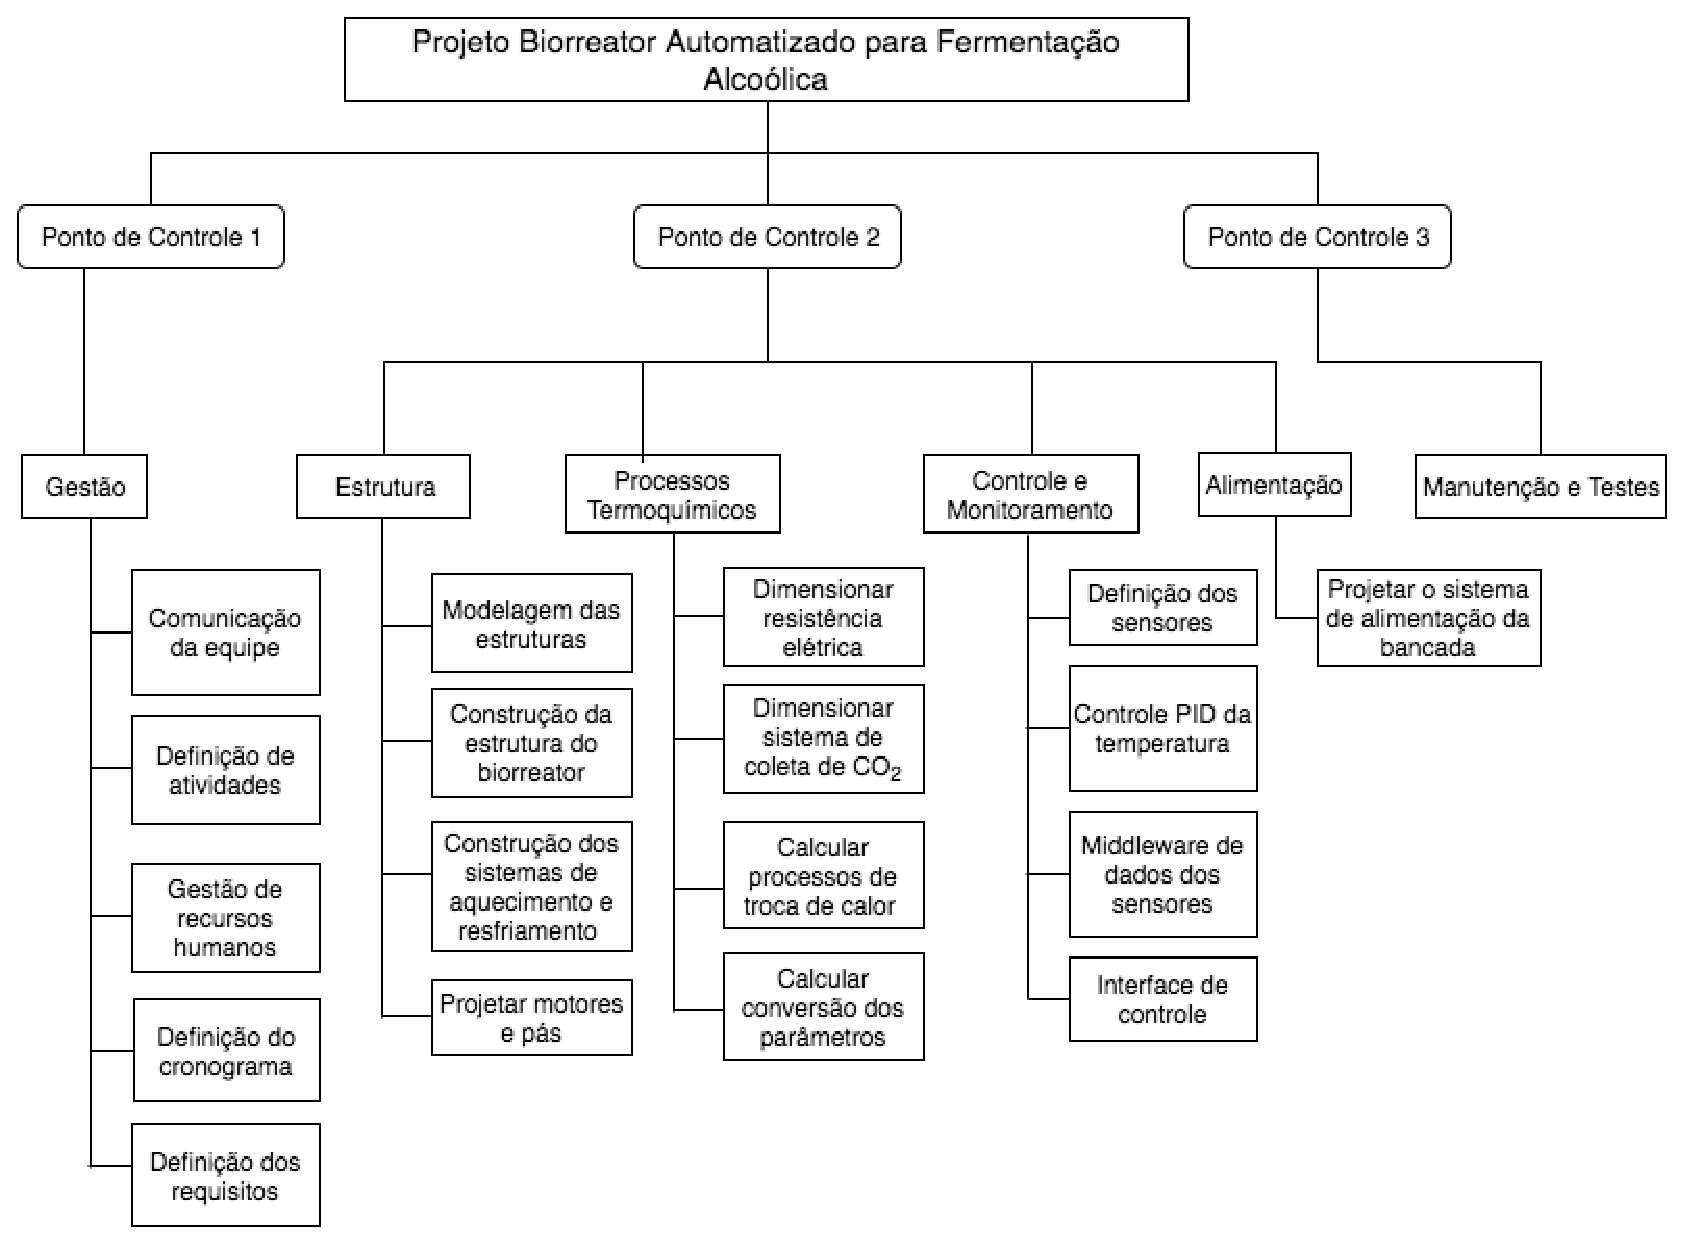
\includegraphics[keepaspectratio=true,scale=0.8, width=\textwidth]{figuras/eap.eps}
	\caption{Estrutura Analítica do Projeto}
	\label{eap}
\end{figure}

\subsection{Tempo}

Baseado nos prazos de entrega nos pontos de controle, foi feito o seguinte cronograma de atividades:

\subsection{Custos}

O gerenciamento dos custos do projeto inclui os processos envolvidos em planejamento, estimativas, orçamentos, financiamentos, gerenciamento e controle dos custos, de modo que o projeto possa ser terminado dentro do orçamento aprovado possuindo foco no custo dos recursos necessários para completar as atividades do projeto.

O gerenciamento dos custos projeto deve considerar também o efeito das decisões de projeto no custo recorrente subsequente do uso, manutenção e suporte do produto, serviço ou resultado do projeto, neste caso ficando limitado a opção da equipe quanto a continuar disponibilizando e oferecendo suporte ao produto final.

A tabela abaixo representa os custos estimados dos materiais selecionados para o desenvolvimento do projeto:

\begin{table}[h]
\centering
\caption{Tabela de custos do projeto}
\resizebox{\textwidth}{!} {
\label{table1}
\begin{tabular}{ll|l|}
\hline
\multicolumn{1}{|l|}{Area}                     & Material                                                                                    & Custo              \\ \hline
\multicolumn{1}{|l|}{ESTRUTURA}                & Conformação mecânica (calandragem) cilíndrica, cônica para aço inoxidável e flange (1,5 mm) & R\$332,00          \\ \hline
\multicolumn{1}{|l|}{}                         & Soldagem inox                                                                               & R\$300,00          \\ \hline
\multicolumn{1}{|l|}{}                         & Tubo de Suporte                                                                             & R\$130,00          \\ \hline
\multicolumn{1}{|l|}{}                         & Tampa flangeada (3 mm)                                                                      & R\$ 120,00         \\ \hline
\multicolumn{1}{|l|}{}                         & Válvula de alívio de pressão                                                                & R\$ 11,15          \\ \hline
\multicolumn{1}{|l|}{}                         & Manômetro                                                                                   & R\$ 37,00          \\ \hline
\multicolumn{1}{|l|}{}                         & 11 Anéis de vedação em silicone (espude)                                                    & R\$ 20,00          \\ \hline
\multicolumn{1}{|l|}{}                         & 2 Torneiras                                                                                 & R\$ 20,00          \\ \hline
\multicolumn{1}{|l|}{}                         & Rotor e Pás                                                                                 & R\$ 50,00          \\ \hline
\multicolumn{1}{|l|}{}                         & Motor                                                                                       & R\$ 300,00         \\ \hline
\multicolumn{1}{|l|}{}                         & Rolamentos                                                                                  & R\$ 10,00          \\ \hline
\multicolumn{1}{|l|}{CONTROLE E MONITORAMENTO} & Sensor Ultrassônico HC-SR04                                                                 & R\$ 15,00          \\ \hline
\multicolumn{1}{|l|}{}                         & 2 Sensores DS18B20 para temperatura                                                         & R\$ 20,40          \\ \hline
\multicolumn{1}{|l|}{}                         & 2 sensores MPX5700DP                                                                        & R\$ 123,00         \\ \hline
\multicolumn{1}{|l|}{}                         & Gravity Analog pH Meter Kit                                                                 & R\$ 147,00         \\ \hline
\multicolumn{1}{|l|}{}                         & Motor de Passo 28BYJ-48 + Driver ULN2003                                                    & R\$ 20,00          \\ \hline
\multicolumn{1}{|l|}{}                         & Conversor A/D ADS1115                                                                       & R\$ 24,00          \\ \hline
\multicolumn{1}{|l|}{}                         & Raspberry PI 3                                                                              & R\$ 200,00         \\ \hline
\multicolumn{1}{|l|}{PROCESSOS TERMOQUÍMICOS}  & Resistência elétrica 5000 W 220 V                                                           & R\$ 100,00         \\ \hline
\multicolumn{1}{|l|}{}                         & Bomba de circulação 220 V                                                                   & R\$ 250,00         \\ \hline
\multicolumn{1}{|l|}{}                         & Mangueira de silicone                                                                       & R\$ 14,00/m        \\ \hline
\multicolumn{1}{|l|}{}                         & Alga chaetomorpha                                                                           & R\$ 34,90          \\ \hline
\multicolumn{1}{|l|}{}                         & Válvula de esfera para gás borboleta fêmea                                                  & R\$ 30,00          \\ \hline
\multicolumn{1}{|l|}{ALIMENTAÇÃO}              & Cabo de Força 3m                                                                            & R\$ 25,00          \\ \hline
                                               &                                                                                             & TOTAL: R\$2.419,55 \\ \cline{3-3}
\end{tabular}
}
\end{table}

\subsection{Alocação de recursos humanos}

A equipe do projeto é formada por 12 membros que foram divididos de acordo com as macro atividades que serão realizadas. Em cada uma delas foi escolhido um membro líder responsável pela supervisão das atividades. Além disso, foi escolhido um líder geral, o gerente do projeto, responsável pela integração de todas as partes do mesmo, e um outro gerente responsável pelo controle de qualidade das atividades. Abaixo se tem a relação esquemática da divisão adotada.

\begin{figure}[h]
	\centering
	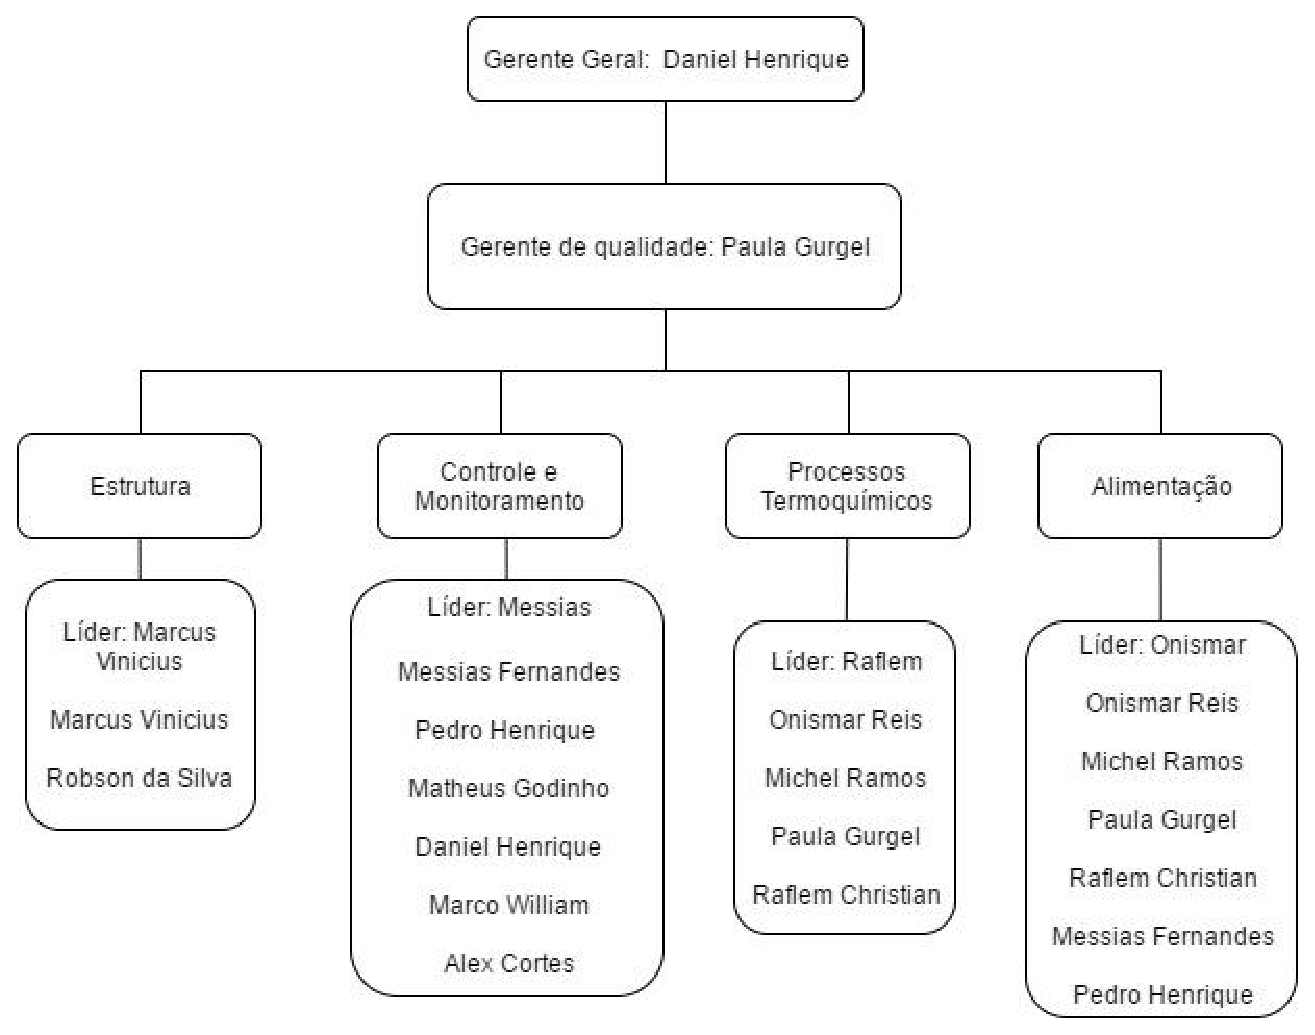
\includegraphics[keepaspectratio=true,scale=0.5]{figuras/divisao.eps}
	\caption{Divisão de frentes de trabalho e gerentes do projeto}
	\label{divisao}
\end{figure}

\subsection{Riscos}

Um plano de gerenciamento de riscos é necessário para calcular o impacto dos riscos no projeto e medidas de contingência para o controles dos mesmos. O plano de gerenciamento de riscos está disponível no anexo A.

\subsection{Requisitos}

A partir da concepção e validação do solucionamento do sistema, os requisitos foram definidos a partir de cada subsistema deste presente projeto.

\begin{itemize}
\item O biorreator deverá ser capaz de aquecer e resfriar dentro da faixa de 0º a 100º Celsius.
\item Ter um sistema que seja capaz de coletar CO2.
\item O rotor do sistema deverá manter-se a uma velocidade constante e pré-determinada.
\item O biorreator deverá possuir dimensões capazes de acomodar os sensores e demais componentes internos definidos no projeto.
\item Quanto a estrutura do biorreator, deverá possuir em sua composição, material favorável quanto a assepsia que o sistema necessita.
\item A dimensão da estrutura do biorreator deverá estar de conformidade com um equipamento de bancada de um laboratório.
\item O biorreator deverá possuir um motor, conectado ao seu rotor, para que a agitação mecânica seja realizada.
\item O biorreator deverá ser automatizado o suficiente para realizar a coleta de dados dos principais parâmetros e gerar gráficos.
\item O biorreator deverá realizar a leitura de dados referente a temperatura, pH, densidade e volume.
\item O biorreator deverá possuir um compartimento, especificamente de açúcar, para se auto-alimentar, quando necessário.
\item O biorreator deverá possuir uma válvula para realizar a coleta da levedura.
\item O biorreator deverá possuir uma válvula de precaução em caso de um aumento de pressão.
\item O biorreator deverá ter um sistema de aquecimento interligado a um controlador PID (Proporcional, Integral e derivativo).
\item Todo o sistema do biorreator deve estar conectado a um sistema de software e  hardware, que o usuário possa ver e controlar todos os parâmetros do mesmo.
\end{itemize}

\subsection{Controle e Monitoramento}

Dada a especificação do projeto, pretende-se realizar medições eletrônicas de valores de temperatura, densidade e potencial hidrogênico(pH). A partir, disso seria utilizado uma unidade microcontrolada para processamento de dados.

Com relação a unidade de controle e aquisição de dados para o monitoramento do sistema será atacado em duas frentes. A primeira solução adotada para este problema será usar uma \textit{Raspberry PI 3}, para realizar a aquisição e processamento de dados, para exercer essa atividade deve-se desenvolver uma biblioteca para cada sensor, com o auxílio de conversores analógicos/digitais para facilitar a recepção de dados pela Raspberry, essa solução pretende reduzir os itens envolvidos no projeto. Em paralelo será trabalhado uma solução alternativa, onde os dados enviados pelos sensores serão recebidos por um microcontrolador Arduino ATMEGA 238, e o dados serão processados e enviados para uma \textit{Raspberry PI 3}, através de um protocolo de comunicação \textit{UART}, para receber e realizar o processamento de dados.

\subsubsection{Medição de temperatura}

Para realizar medições de temperatura foi escolhido o sensor DS18B20, Com relação às suas especificações elétricas, este possui uma variação de tensão de alimentação nos seus pinos de -0.5 a +6V e a faixa de variação na escala de temperatura permite medições que variam de -55ºC a +125ºC. Esta escala de variação é adequada para a medição de valores de temperatura, já que o valor máximo para valores seria de aproximadamente 100ºC no interior do biorreator.

Sobre a precisão do componente, os valores de saída são discretizados na em 8 bits. Ou seja, os 180 valores possíveis de medição são exibidos com precisão de 0,703125ºC. O sensor além disso, possui características à prova de água, devido ao seu encapsulamento, o que facilita a imersão no interior do biorreator.

\begin{figure}[h]
	\centering
	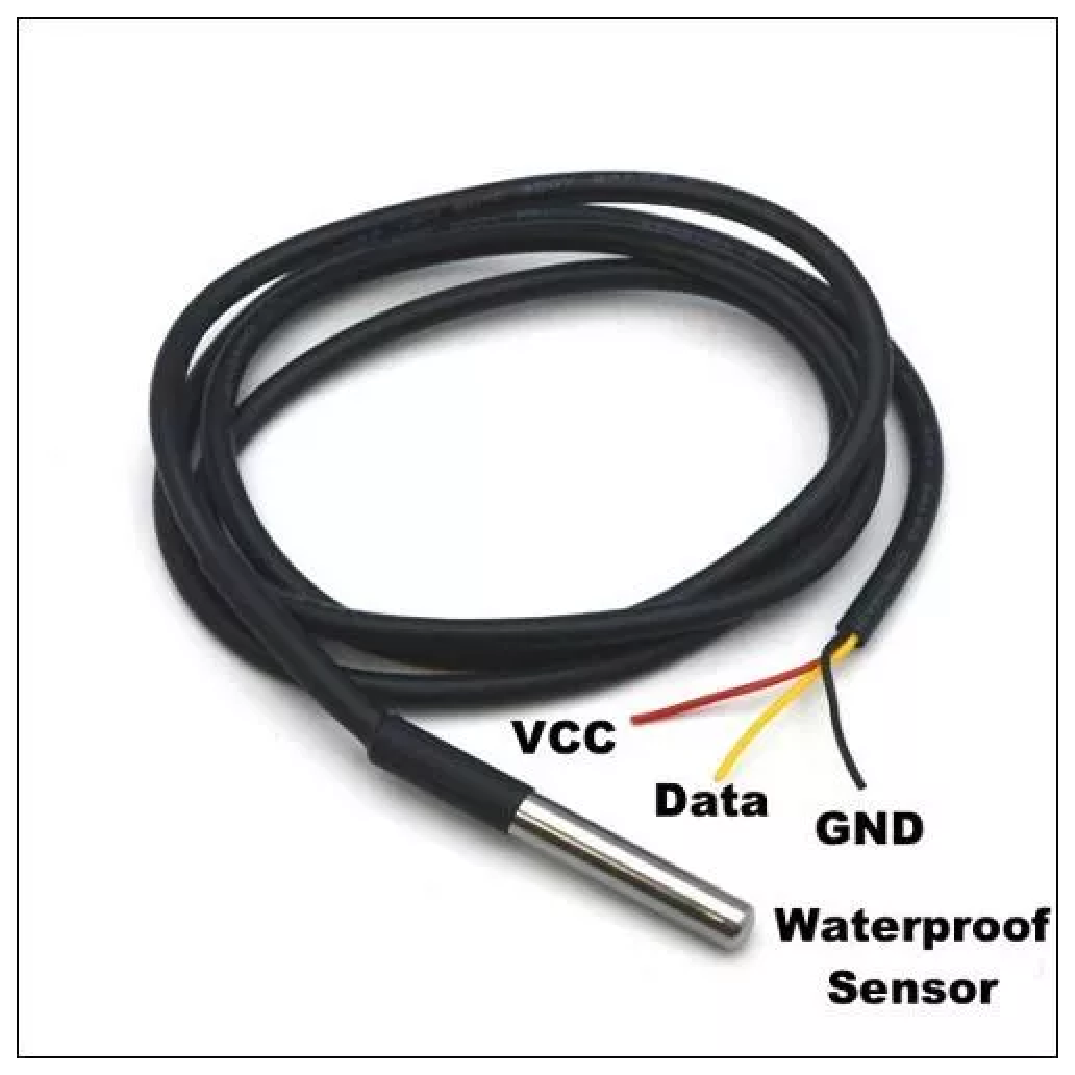
\includegraphics[keepaspectratio=true,scale=0.3]{figuras/probe.eps}
	\caption{Probe para imersão em fluidos}
	\label{probe}
\end{figure}

\subsubsection{Medição de densidade}

A definição da densidade no projeto \nocite{ADS1115} é um requisito para provar a funcionalidade do projeto, torna-se necessário a sua medição. Considerando que o uso de um sensor de densidade é inviável de medição, usa-se o princípio da medição de pressão diferencial para estimar o valor da densidade através da manipulação da equação de Bernoulli. A especificação da medição de densidade, torna-se necessário o uso de sensores de pressão aplicados em dois pontos distintos no interior do biorreator.

\begin{figure}[h]
	\centering
	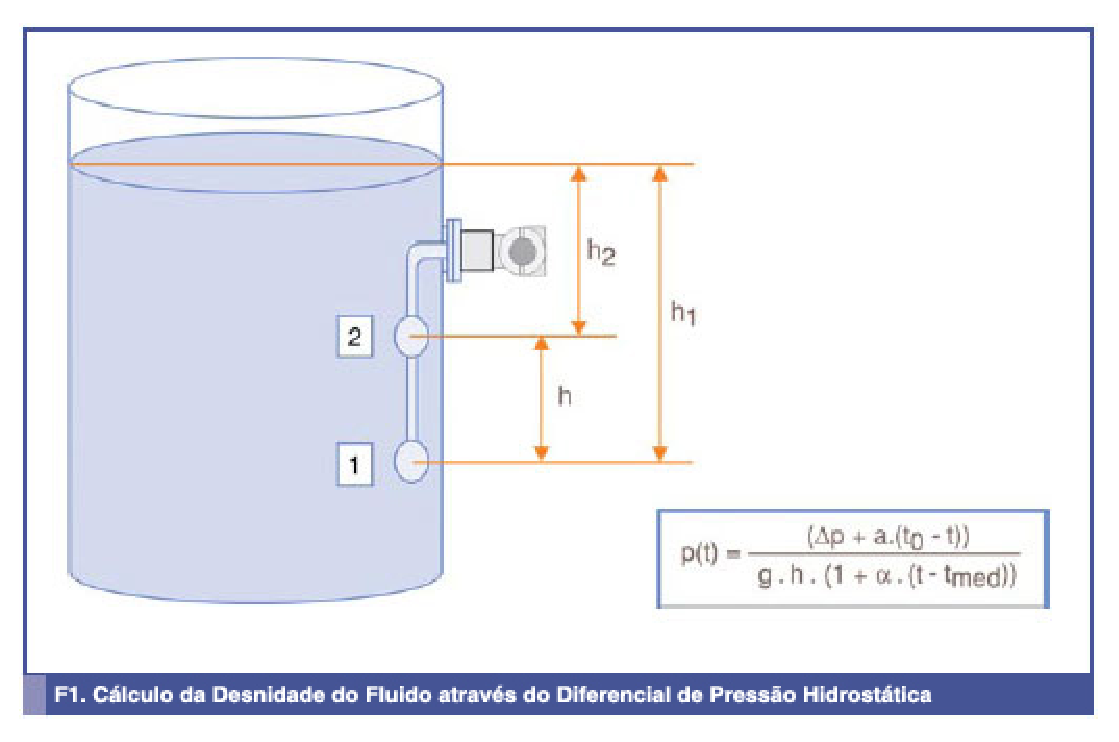
\includegraphics[keepaspectratio=true,scale=0.4]{figuras/densidade.eps}
	\caption{Modelo de cálculo da densidade de um fluido por pressão diferencial}
	\label{densidade}
\end{figure}

Com relação ao coeficientes e parâmetros matemáticos tem-se:

\begin{itemize}
\item \( \rho \): Densidade
\item t: Temperatura do processo
\item \( \Delta \)P: Diferença de Pressão
\item a: Coeficiente de compensação de temperatura no fluído
\item tZERO = Temperatura de Calibração do sensor
\item g: Aceleração da gravidade
\item h: Distância entre os pontos de medição
\item \( \alpha \): Coeficiente de dilatação do material da estrutura
\item tMED: Temperatura de medição nos pontos de medição
\end{itemize}

Dada tal necessidade adotou-se ao projeto o sensor MPX5700DP para medição de pressão sua especificações elétricas são:

\begin{itemize}
  \item Faixa de pressão operacional: 15kPa a 700kPa (0.15 ~ 6.9 atm);
  \item Tensão de alimentação: 5V;
  \item Nº de Pinos: 6;
  \item Pinos úteis: 3;
  \item Precisão: V/P: 6.4mV/kPa;
  \item Corrente de suprimento 7mA;
  \item Faixa de temperatura de operação: -40ºC a + 125ºC;
  \item Dimensões (CxLxA): ~29x37x8mm;
\end{itemize}

\subsubsection{Medição de Volume}

Tal componente utiliza sinais ultrassônicos para determinar a distância entre o sensor e um determinado obstáculo. De modo que no projeto em questão, será responsável por determinar a distância entre o sensor e o nível de açúcar presente na válvula, aferindo assim a quantidade de açúcar ali presente e retornando um dado para o servidor. Apresenta a seguinte tabela de especificações: \nocite{28BYJ-48}

\begin{table}[h]
\centering
\caption{Especificações técnicas Sensor HC-SR04}
\resizebox{\textwidth}{!} {
\label{table2}
\begin{tabular}{|l|l|}
\hline
Tensão de Funcionamento                      & 5 V – DC                                              \\ \hline
Corrente de Funcionamento                    & 15 mA                                                 \\ \hline
Frequência de Funcionamento                  & 40 KHz                                                \\ \hline
Intervalo máximo de verificação de distância & 4 m                                                   \\ \hline
Intervalo mínimo de verificação de distância & 2 cm                                                  \\ \hline
ngulo de Detecção                            & 15º                                                   \\ \hline
Sinal de Entrada Trigger                     & 10uS pulso TTL                                        \\ \hline
Sinal de Saída Echo                          & Entrada do sinal de nível TTL e da faixa de proporção \\ \hline
Dimensão                                     & 45-20-15 mm                                           \\ \hline
\end{tabular}
}
\end{table}

\begin{figure}[h]
	\centering
	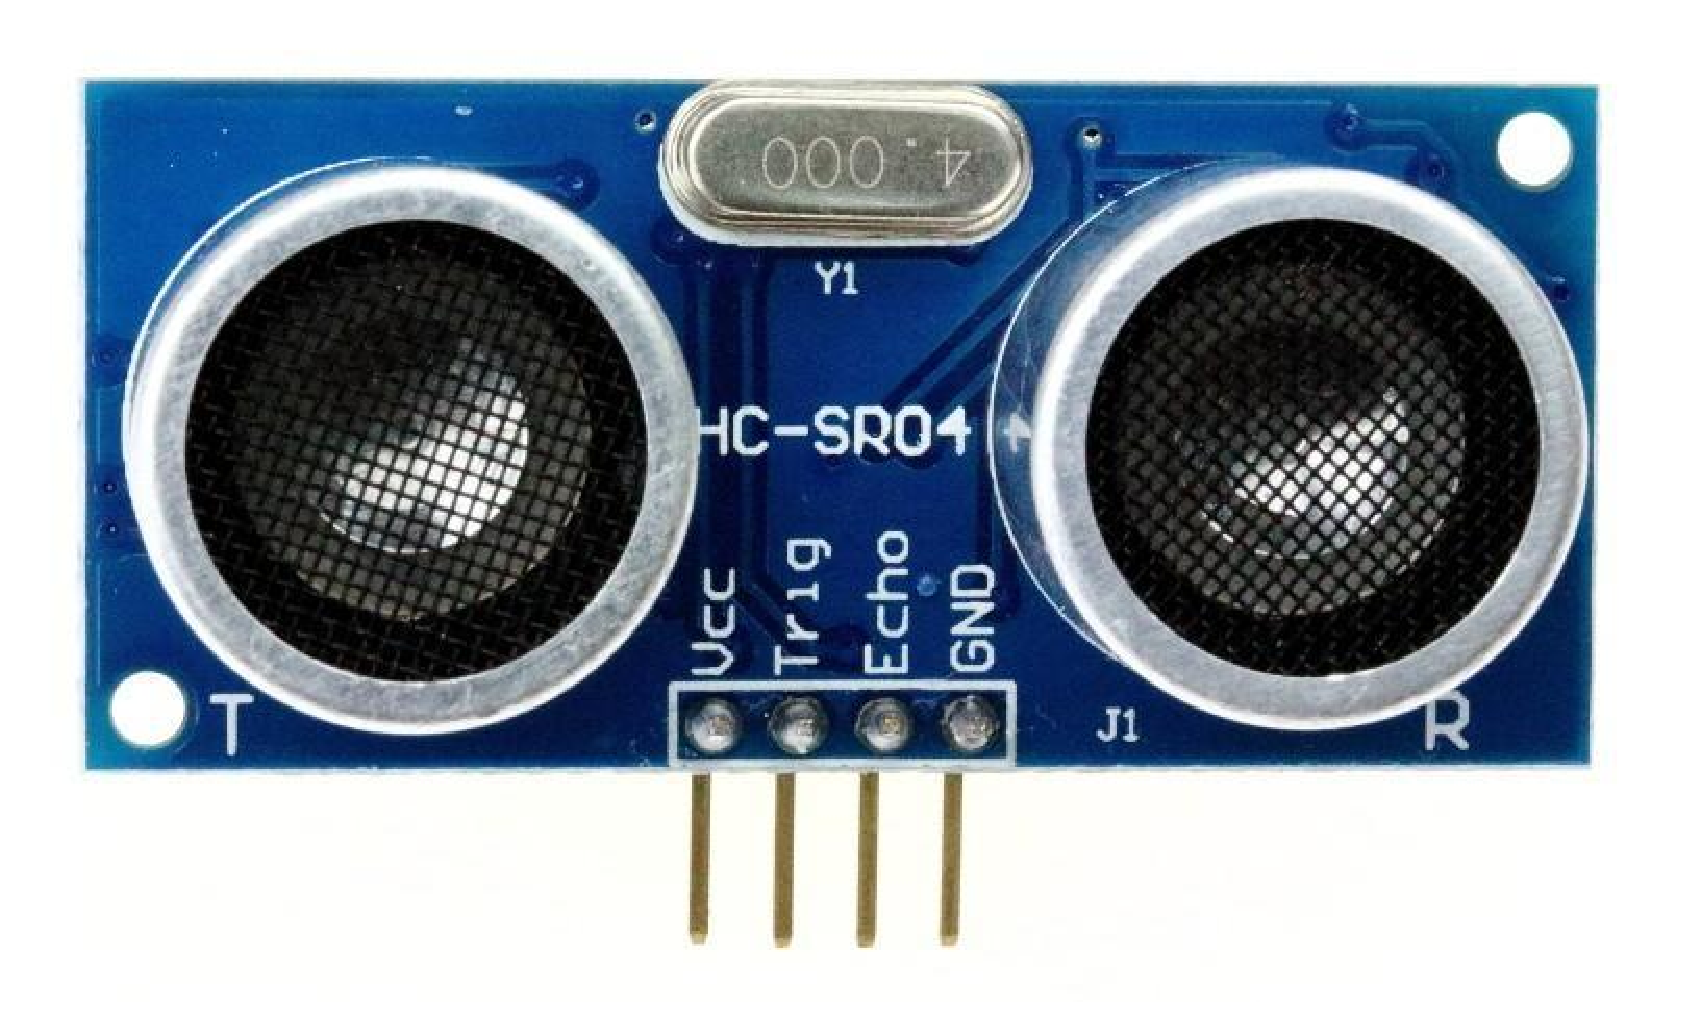
\includegraphics[keepaspectratio=true,scale=0.2]{figuras/sensor1.eps}
	\caption{Ilustração do Sensor HC-SR04}
	\label{sensor1}
\end{figure}

Assim como ilustrado pela imagem acima \nocite{MCP4725} o componente possui 4 pinos (Vcc, Trigger, Echo, GND), onde serão conectados de acordo com as especificações técnicas ditas anteriormente.

\subsubsection{Medição de pH}

  Com relação a especificação da medição de pH, torna-se necessário o uso do kit SKU: SEN0161 que é um kit integrado com um indicador de alimentação, um conector BNC e interface do sensor PH2.0. Segue abaixo a especificação: \nocite{HC-SR04}

\begin{itemize}
  \item Potência do módulo: 5.00V
  \item Tamanho da placa de circuito: 43mm x 32mm
  \item Faixa de medição do pH: 0-14
  \item Temperatura de medição: 0-60 ºC
  \item Precisão: +- 0.1pH (25 ºC)
  \item Tempo de resposta: <=   1min
  \item Sensor de pH com conector BNC
  \item Interface PH2.0 (patch de 3 pés)
  \item Potenciômetro de ajuste de ganho
  \item Indicador de energia LED
\end{itemize}

Calibração do Kit:

\begin{figure}[h]
	\centering
	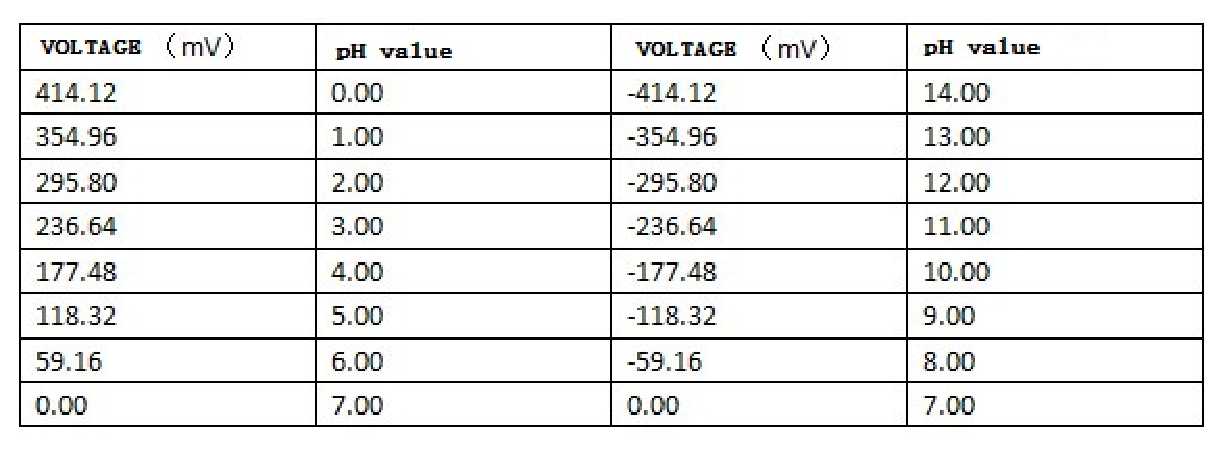
\includegraphics[keepaspectratio=true,scale=0.6]{figuras/ph.eps}
	\caption{Voltagem de Saída medida em relação ao pH}
	\label{ph}
\end{figure}

\begin{figure}[h]
	\centering
	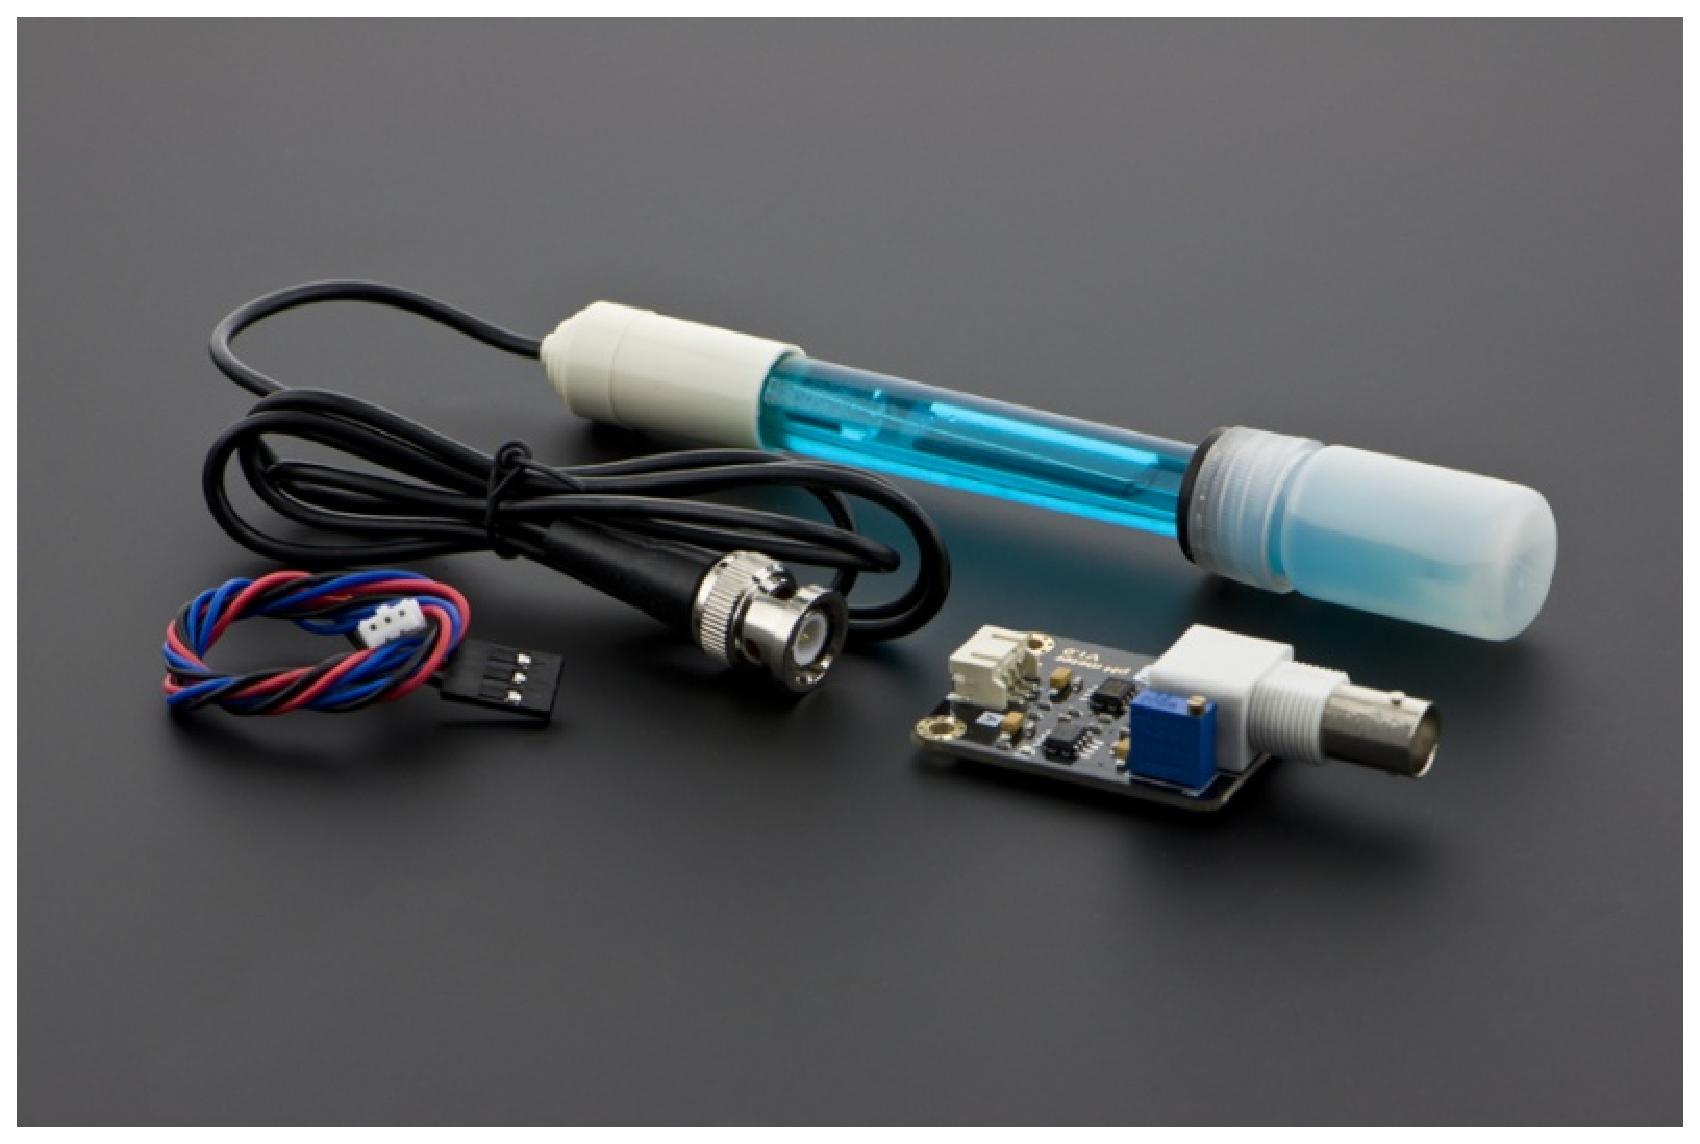
\includegraphics[keepaspectratio=true,scale=0.3]{figuras/sensorph.eps}
	\caption{Kit a ser adotado para medição de pH.}
	\label{sensorph}
\end{figure}

\subsubsection{Válvula de Liberação de açúcar}

Para realizar a liberação de açúcar em tempos contínuos será utilizado um motor de passos para habilitar o despejo de açúcar na função de válvula. Para isso foi escolhido o componente Motor de Passo 28BYJ-48 + Driver ULN2003. Tal componente utiliza conversão de \nocite{ADS1115} tensão em movimentos rotacionais, de modo a codificar o mesmo de modo a parar em posições específicas. De modo que este elemento será utilizado para o controle da válvula de depósito de açúcar, que quando acionado dá-se o passo necessário para liberação da quantidade de açúcar necessária para dentro do Biorreator. Já o Driver, é um sistema vendido juntamente ao motor, qual permite tal codificação de controle. Observa-se as seguintes especificações: \nocite{SEN0161}

\begin{table}[h]
\centering
\caption{Especificação Motor de Passo 28BYJ-48}
\label{table3}
\begin{tabular}{|l|l|}
\hline
Tensão de Funcionamento & 5 V – DC   \\ \hline
Número de Fases         & 4          \\ \hline
Número de Vias          & 5          \\ \hline
Passos por Volta        & 64         \\ \hline
Torque máximo           & 2.2 Kgf.cm \\ \hline
Ângulo por passo        & 5.625º/64  \\ \hline
Frequência              & 100 Hz     \\ \hline
Diâmetro do Eixo        & 5 mm       \\ \hline
Peso                    & 40 g       \\ \hline
\end{tabular}
\end{table}

\begin{figure}[h]
	\centering
	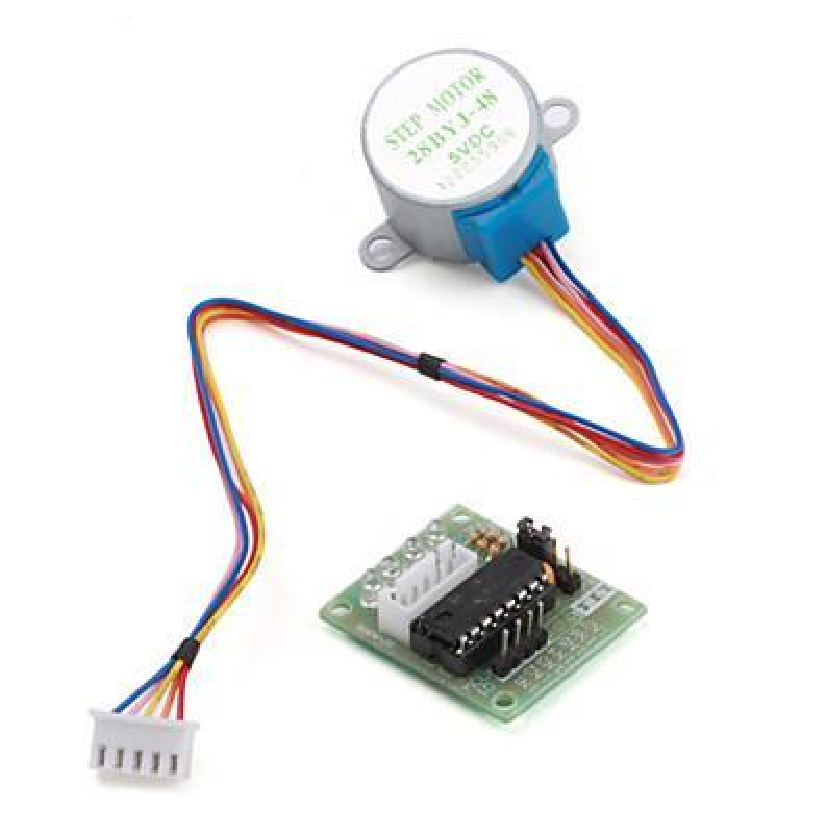
\includegraphics[keepaspectratio=true,scale=0.4]{figuras/sensor2.eps}
	\caption{Motor de Passo 28BYJ-48}
	\label{sensor2}
\end{figure}

\subsubsection{Conversor A/D ADS1115}

Tal componente realiza a conversão de tensão Analógica para Digital. Onde, na aplicação em estudo, será responsável por receber os sinais dos sensores em tensão analógica, converter para digital e encaminhar para o microcontrolador \textit{Raspberry}. Observa-se as seguintes especificações: \nocite{MPX5700}

\begin{table}[h]
\centering
\caption{Especificações Conversor ADS1115}
\label{table4}
\begin{tabular}{|l|l|}
\hline
Tensão de Funcionamento    & 2.0 – 5.5 V (DC) \\ \hline
Canais                     & 4                \\ \hline
Resolução                  & 16 bits          \\ \hline
Frequência de operação SLC & 0.1 -3.4 MHz     \\ \hline
Taxa de Dados              & 8 – 860 SPS      \\ \hline
Dimensões                  & 2 x 1.5 x 0.4 mm \\ \hline
\end{tabular}
\end{table}

\begin{figure}[h]
	\centering
	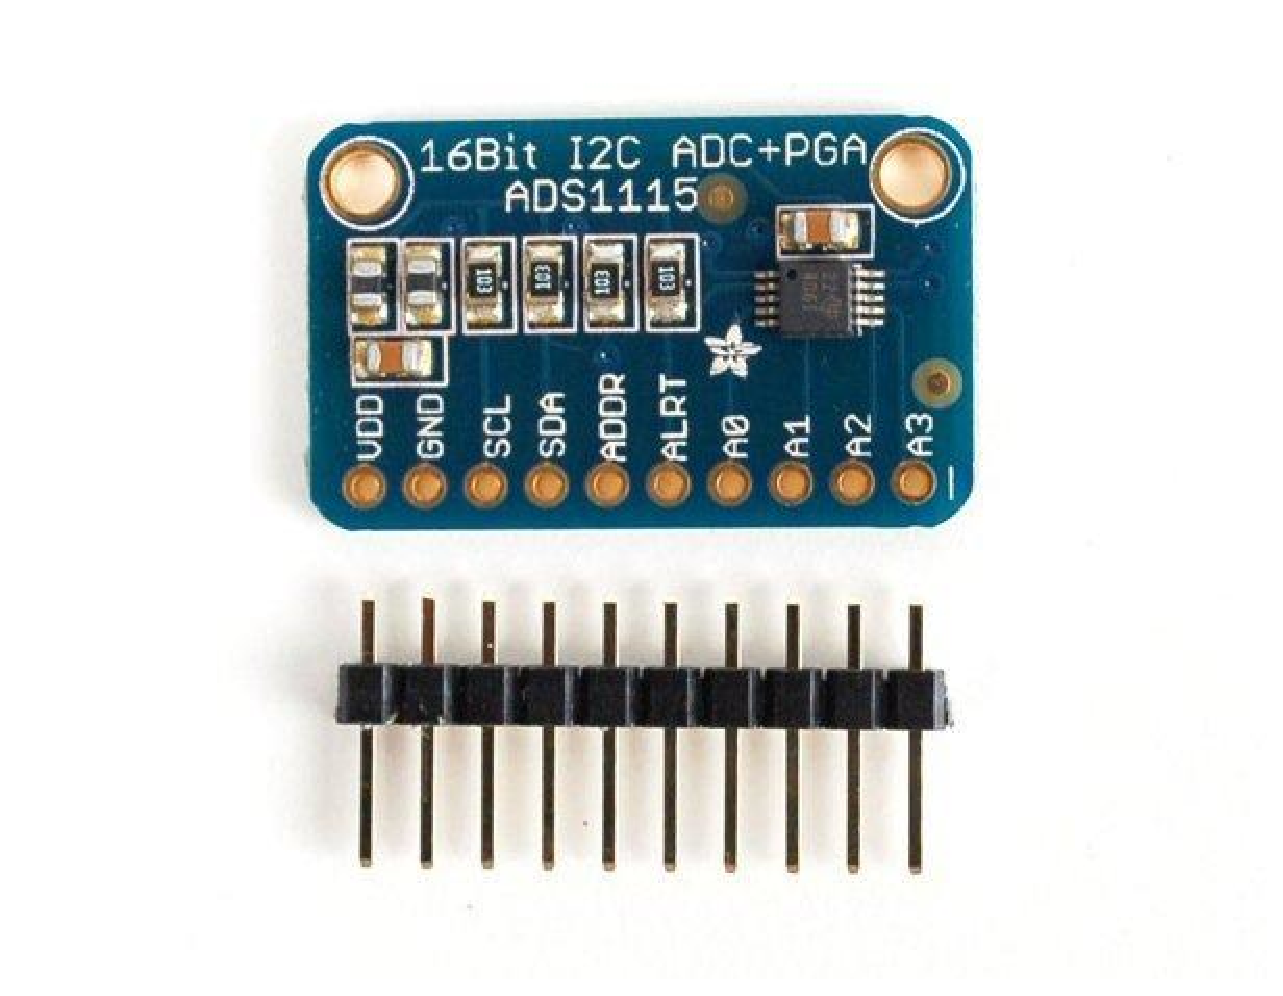
\includegraphics[keepaspectratio=true,scale=0.3]{figuras/sensor3.eps}
	\caption{Conversor ADS1115}
	\label{sensor3}
\end{figure}

\subsubsection{Conversor D/A MCP4725}

Tal componente realiza a conversão de tensão Digital para Analógico. Onde, na aplicação em estudo, será responsável por converter os sinais do cliente/usuário lançados pelo app em tensão digital, quais passam pelo servidor  microcontrolador \textit{Raspberry}, chegam no conversor em questão e são encaminhados para os Atuadores. Observa-se as seguintes especificações:\nocite{ds18b20}

\begin{table}[h]
\centering
\caption{Especificações técnicas Conversor D/A MCP4725}
\label{table5}
\begin{tabular}{|l|l|}
\hline
Tensão de Funcionamento & 2.7 – 5.5 V (DC) \\ \hline
Canais                  & 1                \\ \hline
Resolução               & 12 bits          \\ \hline
\end{tabular}
\end{table}

\begin{figure}[h]
	\centering
	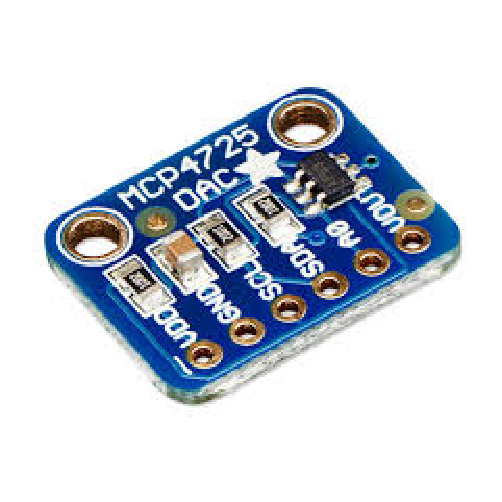
\includegraphics[keepaspectratio=true,scale=0.5]{figuras/sensor4.eps}
	\caption{Conversor D/A MCP4725}
	\label{sensor4}
\end{figure}

\subsubsection{Aplicativo}

Os requisitos do aplicativo foram definidos em formato de \textit{user stories}, identificadas como USXX sendo XX o número da \textit{user story}.

\subsubsubsection{US01}

Eu como usuário desejo visualizar os dados dos sensores para ter um monitoramento da fermentação no biorreator.

Critérios de aceitação:
\begin{itemize}
  \item Dados em forma de gráficos
  \item Gráficos gerados em tempo real
  \item Monitorar sensor de ph
  \item Monitorar sensor de densidade
  \item Monitorar sensor de temperatura
\end{itemize}

Tarefas:
\begin{itemize}
  \item Criar endpoint que disponibiliza os dados pela api
  \item Criar front-end no app para os gráficos
  \item Criar comunicação api-app para capturar os dados
\end{itemize}

\subsubsubsection{US02}

Eu como usuário desejo controlar a temperatura do biorreator para que a fermentação ocorra corretamente do início ao fim.

Critérios de aceitação:
\begin{itemize}
  \item Inserir a quantidade de graus desejada
\end{itemize}

Tarefas:
\begin{itemize}
  \item Criar endpoint para receber dados na api
  \item Criar front-end do app para receber a temperatura
  \item Criar comunicação app-api para enviar dados
\end{itemize}

\subsubsubsection{US03}

Eu como usuário desejo criar uma fermentação para poder diferenciar os dados do aplicativo por fermentação

Critérios de aceitação:
\begin{itemize}
  \item Título
  \item Data de início
  \item Data de término
\end{itemize}

Tarefas:
\begin{itemize}
  \item Criar endpoint para salvar fermentação na api
  \item Criar front-end da criação de fermentação no app
  \item Criar comunicação app-api para salvar fermentação
\end{itemize}

\subsubsubsection{US04}

Eu como usuário desejo controlar a quantidade de açúcar do biorreator para ter um controle do pH.

Critérios de aceitação:
\begin{itemize}
  \item Quantidade de rotações que o motor vai executar
\end{itemize}

Tarefas:
\begin{itemize}
  \item Criar endpoint para receber os dados do controle de açúcar
  \item Criar front-end que recebe a quantidade de rotações do motor no app
  \item Criar comunicação app-api para enviar os dados de quantidade de rotações
\end{itemize}

\subsubsubsection{US05}

Eu como usuário desejo gerar um relatório sobre uma determinada fermentação para ver o que aconteceu de certo e errado.

Critérios de aceitação:
\begin{itemize}
  \item Gerar relatório em pdf
  \item Gerar relatório no próprio aplicativo
\end{itemize}

Tarefas:
\begin{itemize}
  \item Gerar endpoint que enviará todos os dados do relatório
  \item Gerar estrutura do pdf
  \item Fazer front-end do relatório no app
  \item Fazer comunicação de dados app-api
  \item Gerar pdf
\end{itemize}

\subsubsubsection{US06}

Eu como usuário desejo receber notificações com os status do biorreator para monitorar sem o aplicativo estar aberto.

Critérios de aceitação:
\begin{itemize}
  \item Push notification quando finalizar o processo
  \item Push notification quando algum sensor apresentar dados suspeitos
\end{itemize}

Tarefas:
\begin{itemize}
  \item Configurar serviço de push notification na api
  \item Configurar serviço de push notification no app
  \item Criar momentos de envio da push notification na api
\end{itemize}

\section{Especificação do biorreator}

\subsection{Estrutura}

O intuito inicial do projeto seria em adotar normas para vasos de pressão, sendo estas a Norma Regulamentadora 13, de aplicação nacional, e a norma regulamentada pela ASME \textit{(American Society of Mechanical Engineers)}, porém devido a falta de recursos financeiros para seguí-los, os docentes sugeriram formular o projeto como um protótipo. O protótipo foi formulado no CATIA como prévia para fabricação, sendo passível de alterações futuras.

O material adotado no projeto para o desenvolvimento do alicerce do biorreator foi o aço inoxidável 304 devido a diversos motivos, como o alto grau de pureza presente na peça em relação aos demais aços, sendo que esta pureza se torna necessária pertinente a fermentação que ocorrerá, não sendo possível a realização com elementos contaminantes na reação, outro fato se dá a alta condução térmica, aperfeiçoando a troca de calor para uma maior eficiência na transferência de calor do sistema.

As chapas metálicas serão adquiridas e remetidas para calandragem, onde tomarão forma cônica e cilíndrica para a adequação  ao projeto. O fundo do tanque com formato esférico foi cogitado, mas diante a dificuldade em conformar a peça tornou-se impraticável sua produção.

As figuras abaixo ilustram a modelagem realizada para ter como ponto de partida o desenvolvimento estrutural do biorreator.

\begin{figure}[h]
	\centering
	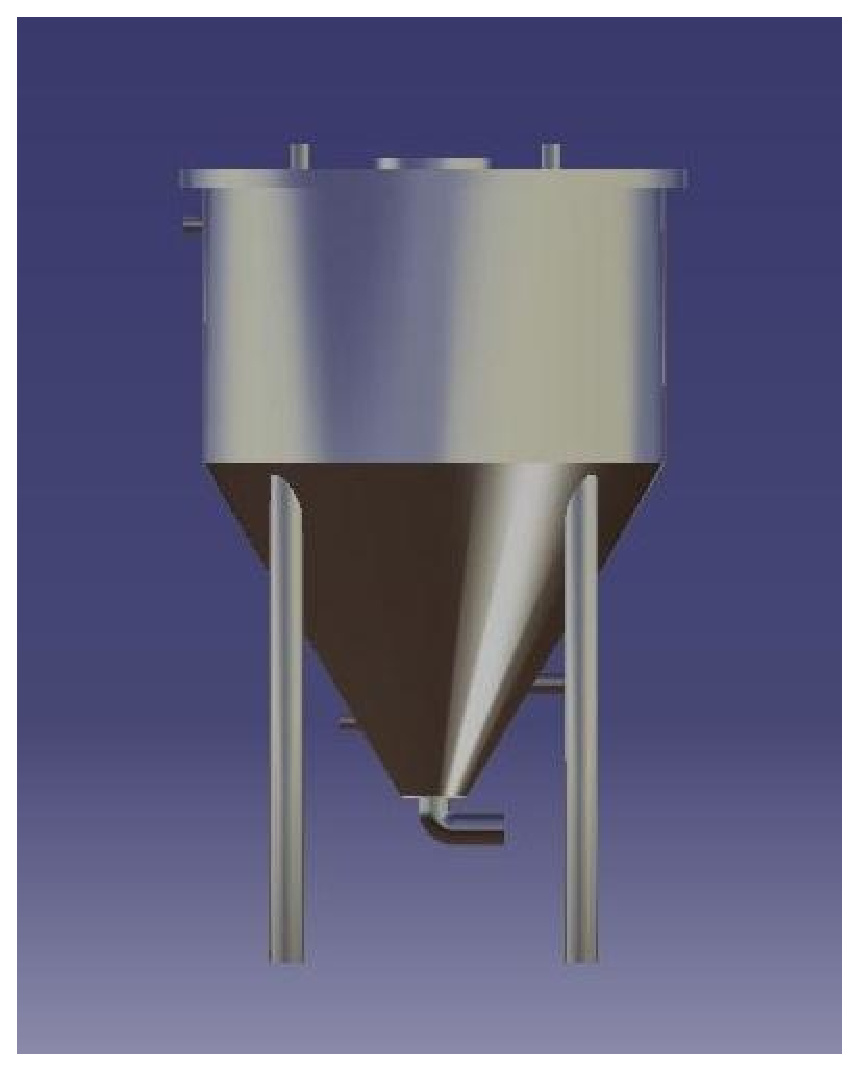
\includegraphics[keepaspectratio=true,scale=0.5]{figuras/catia1.eps}
	\caption{Biorreator modelado no CATIA - Posição 1}
	\label{catia1}
\end{figure}

\begin{figure}[h]
	\centering
	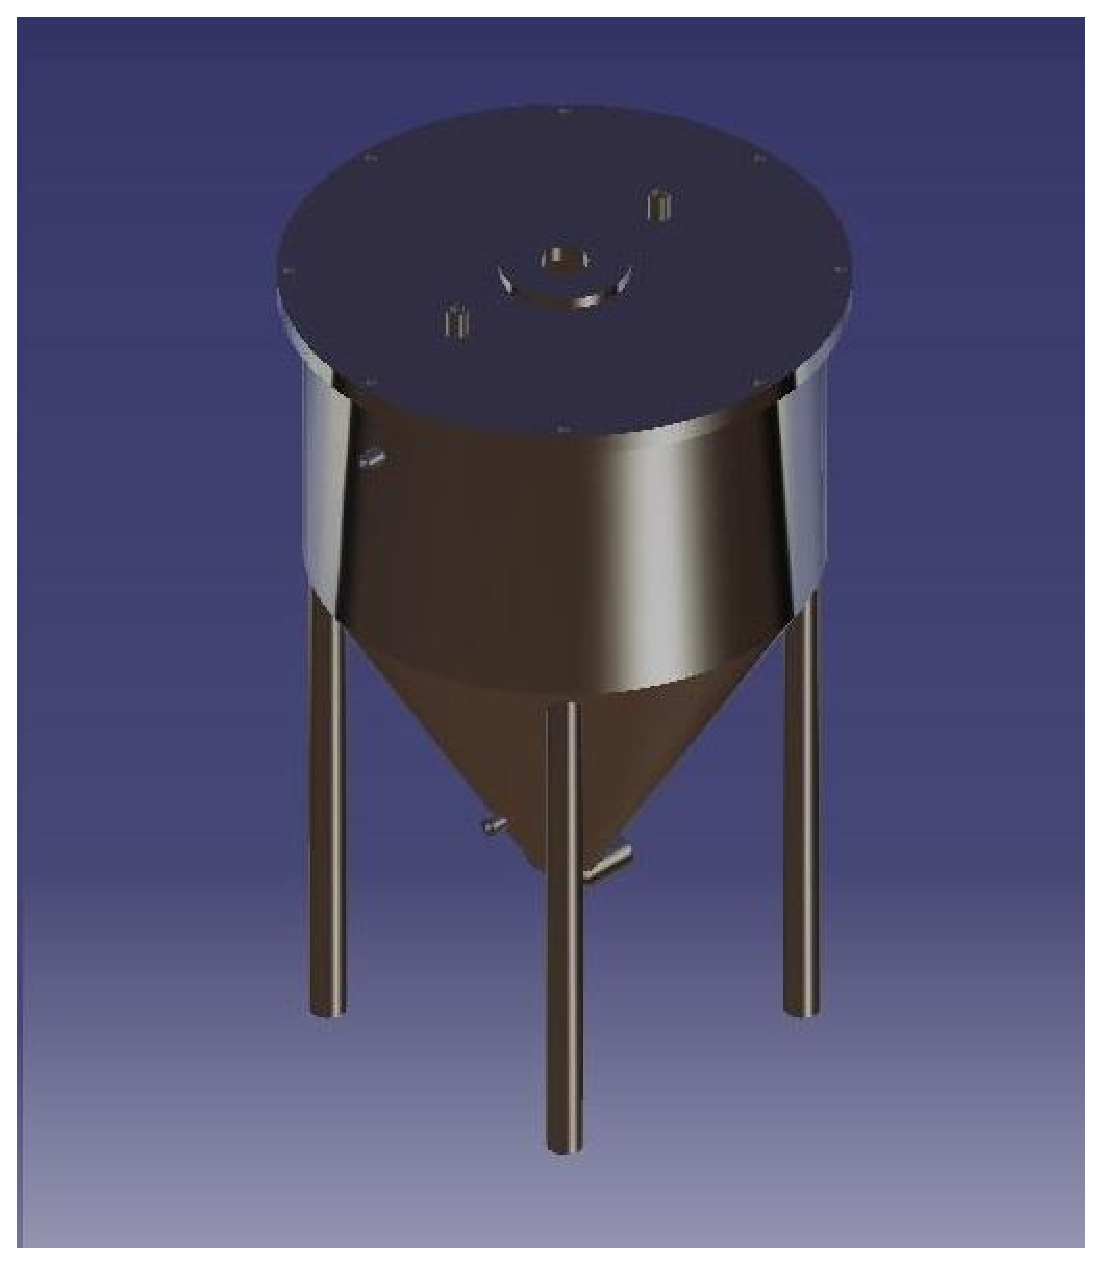
\includegraphics[keepaspectratio=true,scale=0.4]{figuras/catia2.eps}
	\caption{Biorreator modelado no CATIA - Posição 2}
	\label{catia2}
\end{figure}

A modelagem será feita com possíveis correções entre o ponto de controle 1 e 2, para então ser utilizado um software para simulação térmica do biorreator no  \textit{ANSYS}.

\subsubsection{Eixo}

Eixos são elementos que transmitem potência ou movimento. Um projeto de eixo visa atender a critérios de rigidez e deflexão, de resistência estática e à fadiga, além de uma análise de suas velocidades críticas. \cite{shigley2005projeto}

O critério de rigidez visa atender uma inclinação máxima que o eixo possa ter na região dos mancais. Essa inclinação máxima depende dos tipos de rolamentos empregado. Para atender os critérios de resistência existem cinco critérios de falha mais comuns e são eles: Langer, Sodeberg, Goodman, DE-Gerber e ASME-elíptico. A Figura 1 mostra as curvas desses quatro critérios em função das tensões estáticas (\( \sigma \)e) e alternadas (\( \sigma \)a) atuando no eixo. \cite{shigley2005projeto}

\begin{figure}[h]
	\centering
	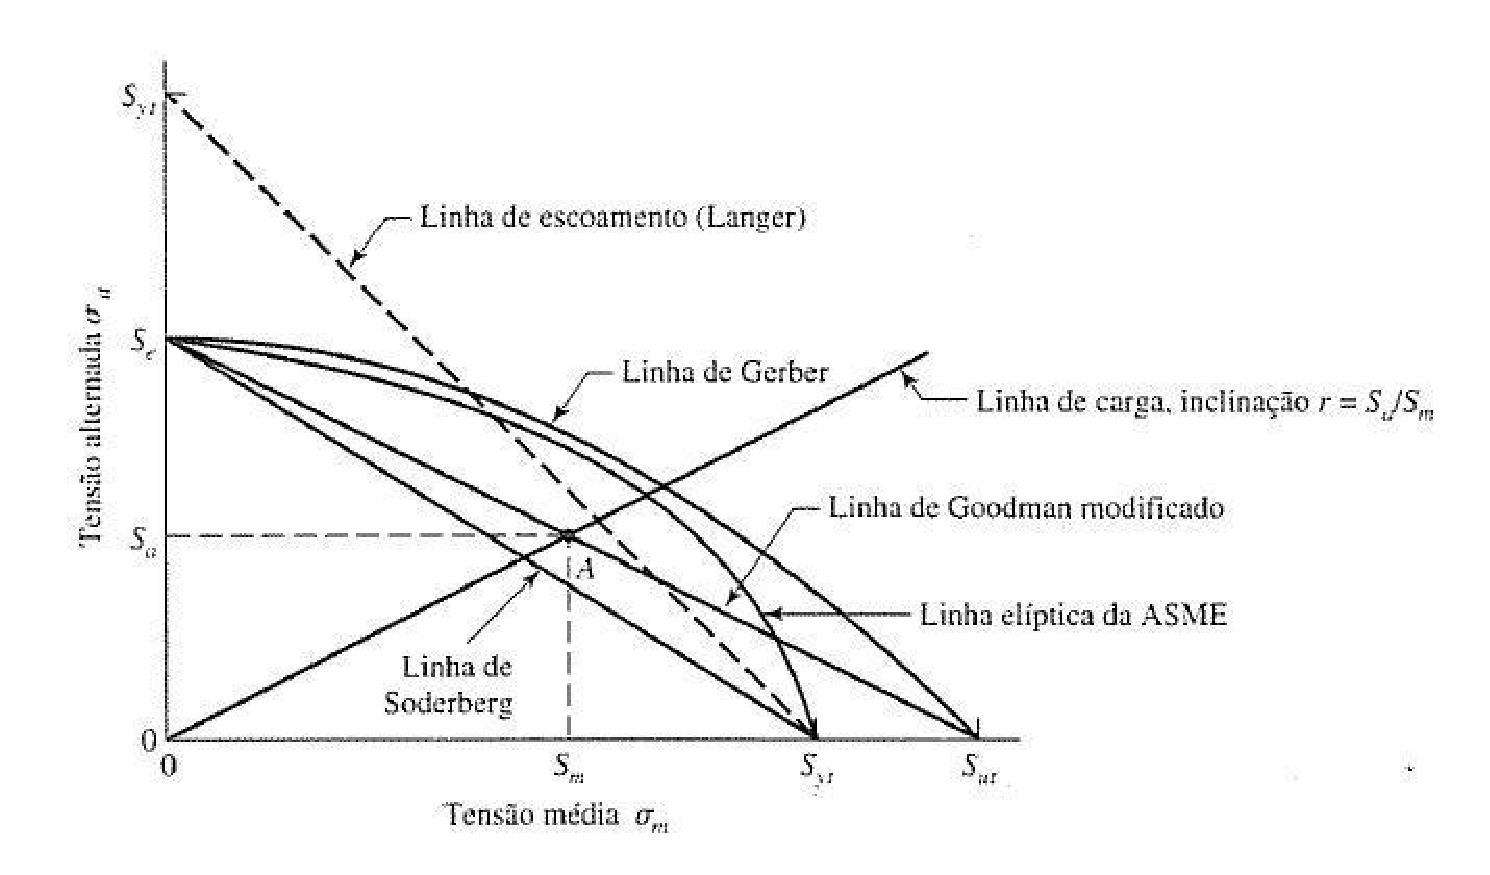
\includegraphics[keepaspectratio=true,scale=0.5]{figuras/eixo.eps}
	\caption{Critérios de falha em fadiga \cite{shigley2005projeto}.}
	\label{eixo}
\end{figure}

Dentre os materiais utilizados para fabricação de eixos, os aços são os materiais mais comuns. Isso se deve ao fato de possuírem um bom módulo de Young, o que se reflete diretamente numa melhora na questão de rigidez. Aços carbono SAE 1020-1050 são escolhas comum, porém quando as solicitações de resistência são muito elevadas alguns aços ligas podem ser utilizados como os SAE 3140, 4140-50, 4340. \cite{shigley2005projeto} Para aplicações em casos especiais, como o de atmosfera corrosiva, pode-se usar também os aços inoxidáveis.  \cite{norton2013projeto}.

O material de eixo a ser adotado para esse projeto é o aço inoxidável 304, por sua aplicabilidade em fermentações com risco de contaminação minimizados e também por conseguir atender os critérios de rigidez e resistência. O critério de resistência a fadiga a ser adotado é o critério de DE-Gerber por ser um critério menos conservador e acarretar em um eixo com um diâmetro menor.

\subsubsection{Rotor}

As pás do rotor serão construídas em material aço inox 304. As especificações para o projeto visa que o impelidor tenha aplicações em velocidade baixa a média, para misturas de baixa e média viscosidade. Os rotores que se inserem nesse perfil seriam rotores de pá cruzada, pá reta, pá pivotante dentre outras.

\begin{figure}[h]
	\centering
	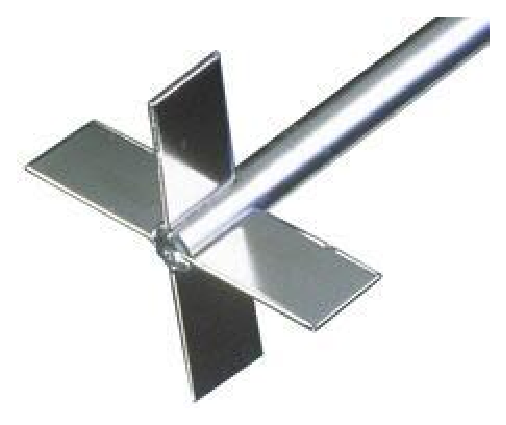
\includegraphics[keepaspectratio=true,scale=0.6]{figuras/pa.eps}
	\caption{Rotor de pá cruzada}
	\label{pa}
\end{figure}

O aço inoxidável 304 é classificado como aço inoxidável austenítico (aços não magnéticos), e possui características que enfatizam no uso para equipamentos na indústria química, depósitos de cerveja, tanques de fermentação, indústria farmacêutica dentre outras, sendo este aço com excelente aspecto para soldabilidade e estampabilidade \cite{kloeckner}.

\subsubsection{Flambagem}

As colunas que sustentam o biorreator sofrem com carregamentos axiais de compressão e podem, portanto, falhar por flambagem. A flambagem depende de diversos fatores, tais como o índice de esbeltez (Sr) das colunas e de suas respectivas condições de contorno. \cite{norton2013projeto}.

O valor do índice de esbeltez é responsável por caracterizar a coluna em coluna curta, a qual essa falhará por compressão, ou nas chamadas colunas longas, onde essa falhará por flambagem. O Sr depende do comprimento (l) da coluna e de propriedades de sua seção transversal, como a área (A) e o menor momento de inércia da seção transversal (I) . O índice de esbeltez é calculado a partir da equação 1. \cite{norton2013projeto}.

\[Sr = 1/\sqrt{\frac{I}{A}}\]

A Figura \ref{solda} mostra diversas condições de contorno e as curvas de deflexão da coluna para cada caso.

\begin{figure}[h]
 \centering
 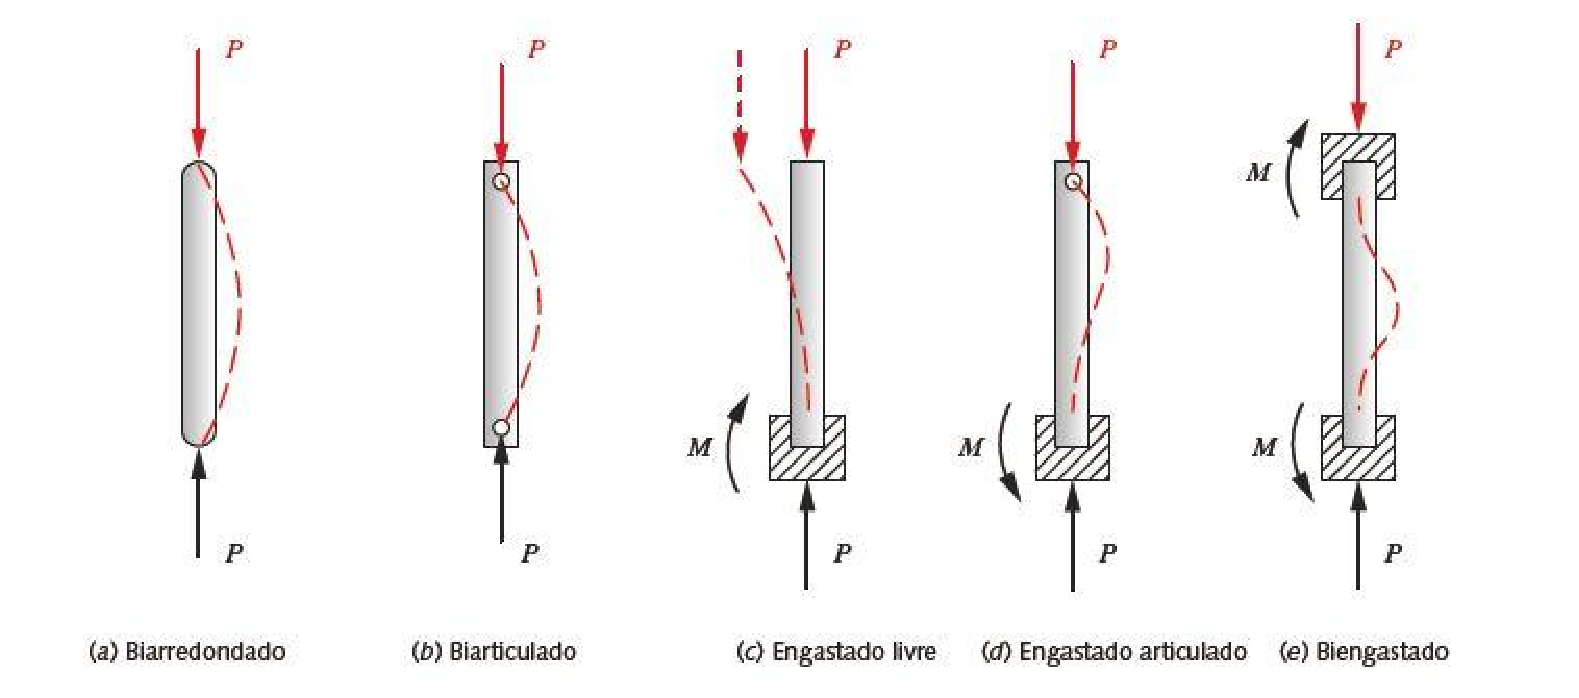
\includegraphics[keepaspectratio=true,scale=0.5]{figuras/solda.eps}
 \caption{Condições de contorno e curvas de deflexão.}
 \label{solda}
\end{figure}

\subsubsection{Soldagem}

Dentre os processos de soldagem mais difundidos na indústria, estão a soldagem a arco, soldagem a gás, soldagem por brasagem, soldagem por resistência e soldagem por laser. Para a soldagem aplicada no biorreator, devido a especificação do uso de aço inoxidável, será empregada a técnica de soldagem a arco. Este processo caracteriza-se pela participação do material base na fusão que constituirá a solda \cite{chiaverini1986tecnologia}.

O processo de soldagem que possibilita soldar a maioria dos metais e ligas, como, aços comuns, aços especiais (caso do aço inoxidável), alumínio, magnésio, cobre dentre outros é conhecido como processo de soldagem a arco com proteção de gás argônio, também chamado de TIG, pertinente ao uso de um eletrodo de tungstênio não consumível. O tungstênio possui a característica de suportar alta intensidade de corrente o que viabiliza o uso para obter grande quantidade de calor em uma área concentrada \cite{chiaverini1986tecnologia}.

\begin{figure}[h]
 \centering
 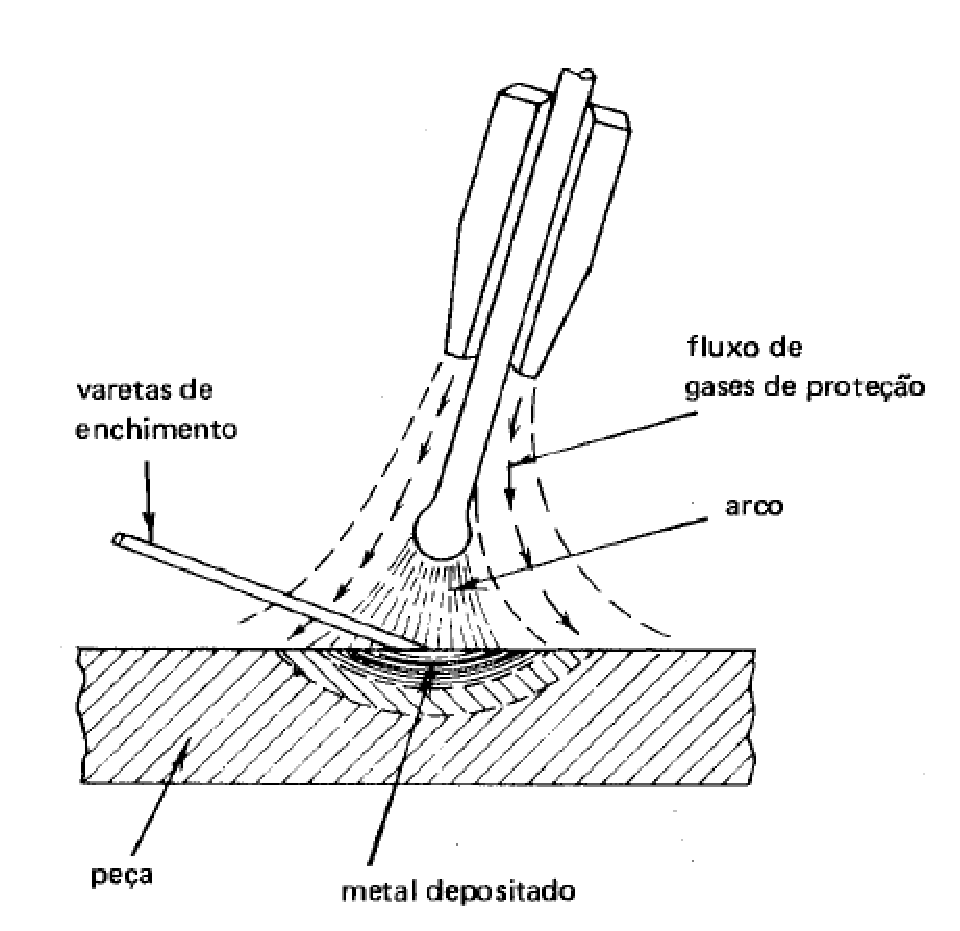
\includegraphics[keepaspectratio=true,scale=0.5]{figuras/contorno.eps}
 \caption{Soldagem por arco com proteção de gás argônio}
 \label{contorno}
\end{figure}

\subsection{Processos Termoquímicos}

A temperatura dentro do biorreator não possui uniformidade em todas as regiões, uma vez que o calor provocado pela fermentação não ocorre a uma taxa constante. Dessa forma, torna-se necessário o uso de múltiplos sensores de temperatura, para um monitoramento mais preciso \cite{silveira2009analise}. Uma das características do biorreator proposto é a variação da temperatura em uma faixa de 0 a 100ºC com controle automático PID no aquecimento. Os sistemas de resfriamento e aquecimento serão separados, uma vez que o resfriamento só ocorrerá ao final da reação com a finalidade de resfriar o mosto para etapas posteriores do processo, ou como medida de segurança para o caso de superaquecimento do biorreator.

\subsubsection{Sistema de resfriamento}

O ciclo de refrigeração é definido como uma região onde o fluido refrigerante circula, permutando em líquido e vapor de forma que viabilize a transferência de calor de um objeto onde ocorre a evaporação, processo que absorve calor, com baixa pressão e temperatura e a condensação, situação a qual rejeita calor, com alta pressão e temperatura. A temperatura dentro do cilindro do biorreator não possui uniformidade em todas as regiões, uma vez que o calor provocado pela fermentação não ocorre a uma taxa constante. Dessa forma, torna-se necessário o uso de múltiplos sensores de temperatura, para um monitoramento mais preciso \cite{silveira2009analise}.

Segundo \cite{mcketta1991heat} os tipos de sistemas de resfriamento estão em escala crescente a seguir

\textbf{Jaqueta Simples:} A jaqueta simples, ou camisa simples, possui de 2 a 3 polegadas de espaço anular na qual o fluido percorre lentamente. Ele é voltado para aplicações com baixa necessidade de transferência de calor.

\begin{figure}[h]
	\centering
	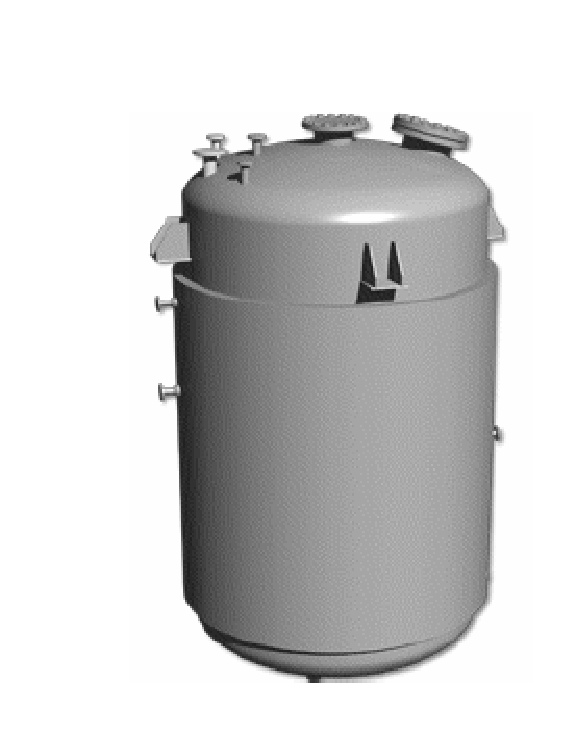
\includegraphics[keepaspectratio=true,scale=0.4]{figuras/jaqueta.eps}
	\caption{Jaqueta simples \cite{silveira2009analise} }
	\label{jaqueta}
\end{figure}

\textbf{Jaqueta com defletores em espiral:} A jaqueta com defletores consiste em um espiral longo de metal que direciona velocidades de fluido um pouco acima em relação as jaquetas simples.

\begin{figure}[h]
	\centering
	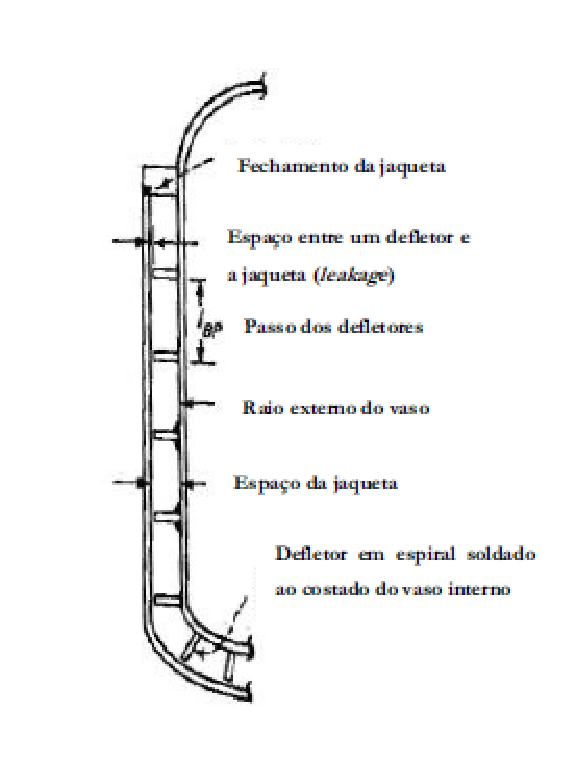
\includegraphics[keepaspectratio=true,scale=0.6]{figuras/jaqueta2.eps}
	\caption{Imagem em corte de jaqueta com defletores\cite{silveira2009analise}}
	\label{jaqueta2}
\end{figure}

\textbf{Jaqueta tipo dimple:} A jaqueta dimple possui a característica de não afetar a resistência sendo construído a partir de materiais mais leves.

\begin{figure}[h]
	\centering
	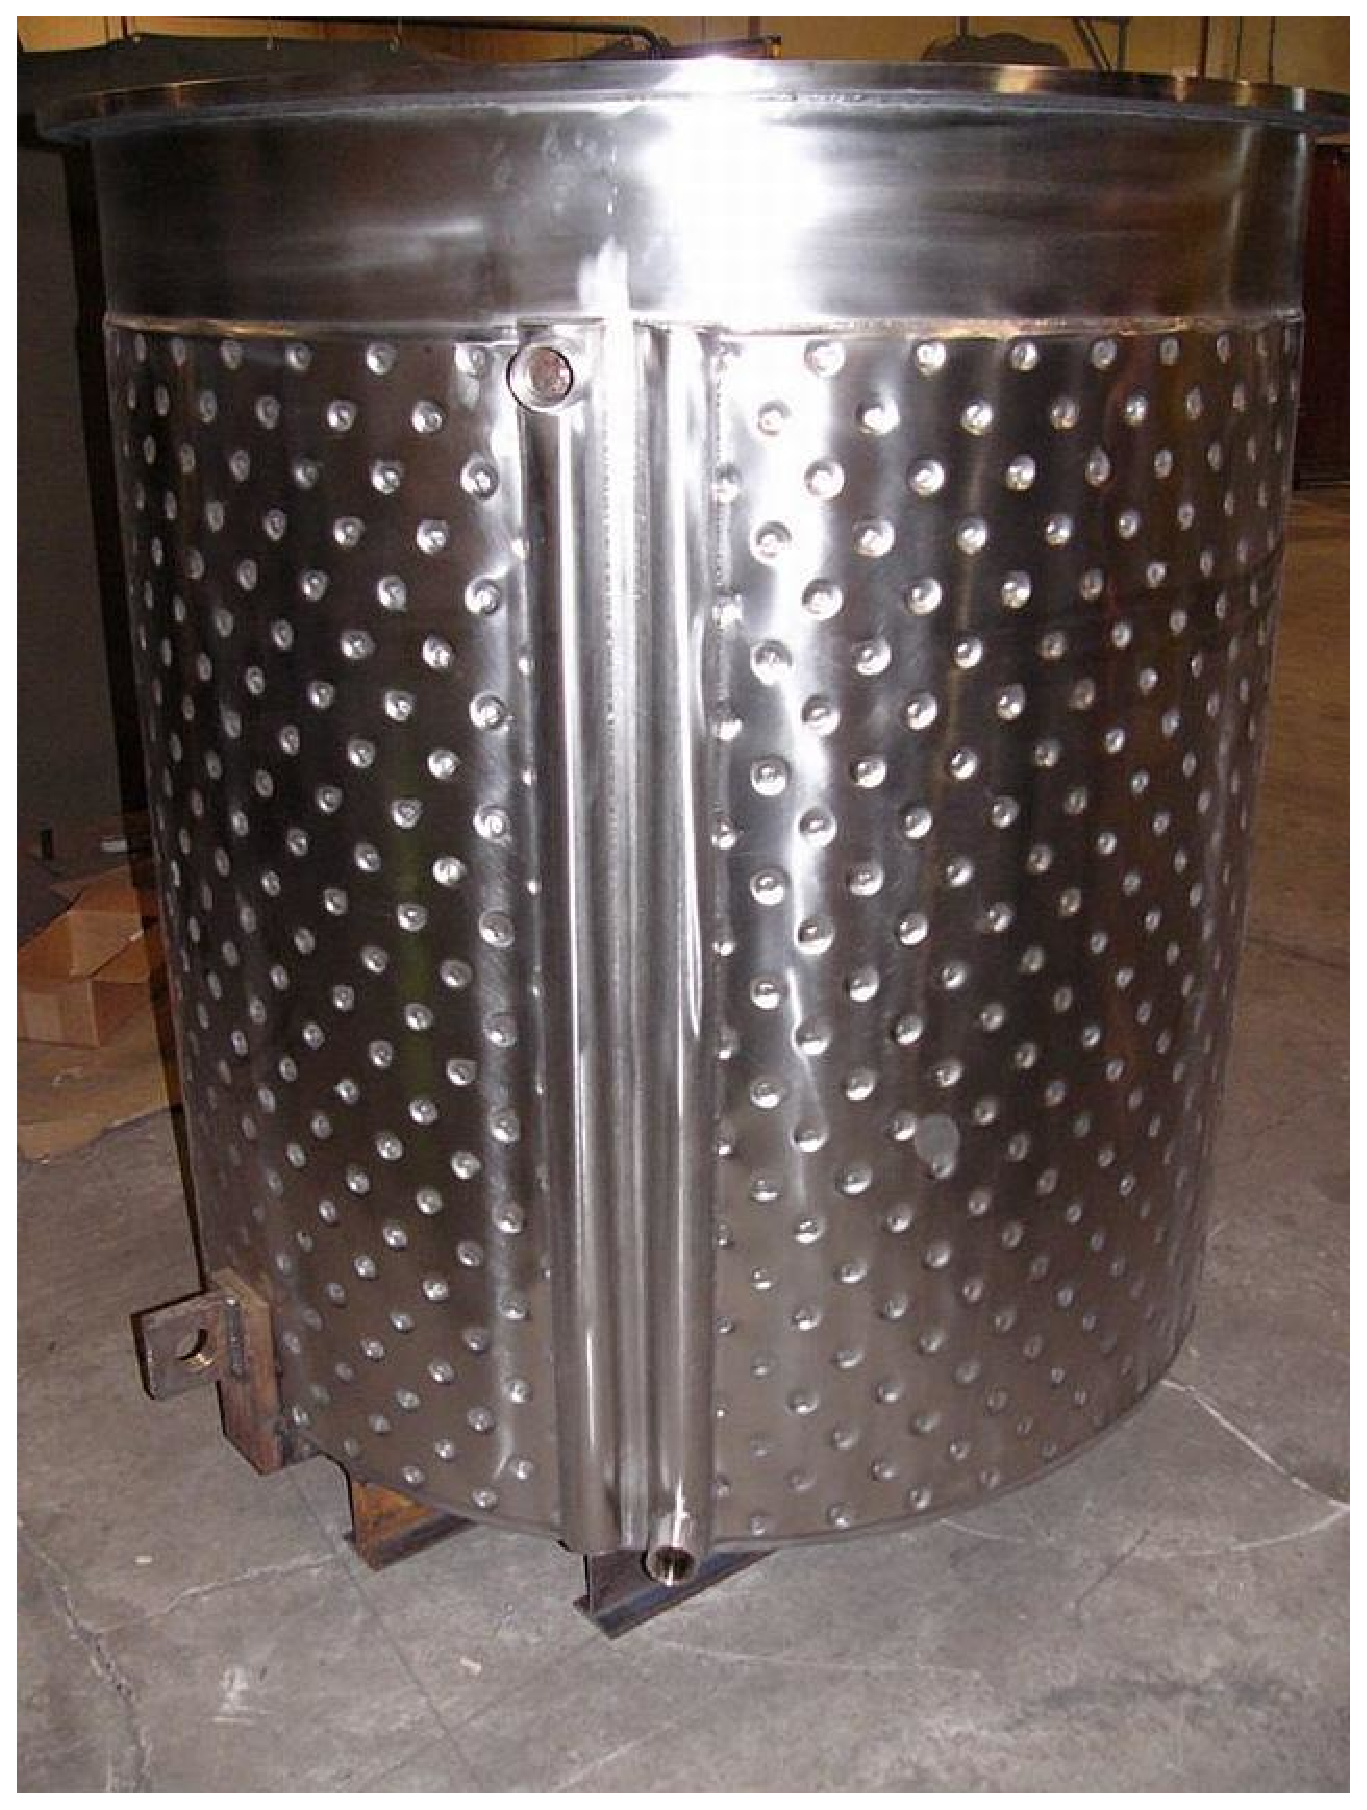
\includegraphics[keepaspectratio=true,scale=0.2]{figuras/jaqueta3.eps}
	\caption{Jaqueta Dimple. Fonte: Royal Welding - Site de Internet}
	\label{jaqueta3}
\end{figure}

\textbf{Jaqueta de serpentina meia-cana:} A jaqueta meia cana eleva a rigidez da estrutura, sendo os tubos soldados a parte externa do vaso.

\begin{figure}[h]
	\centering
	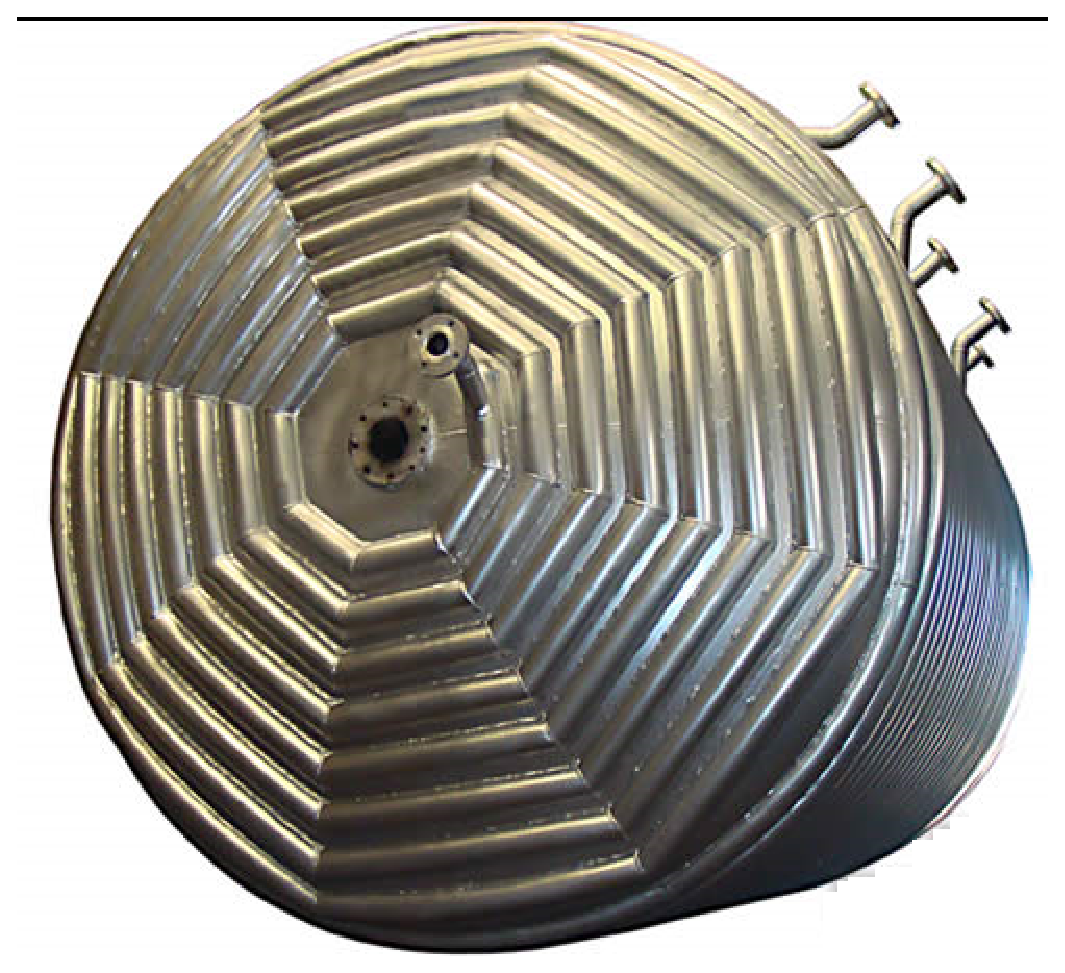
\includegraphics[keepaspectratio=true,scale=0.2]{figuras/jaqueta4.eps}
	\caption{Jaqueta meia-cana. Fonte: Metalúrgica Metalnox - Site de Internet}
	\label{jaqueta4}
\end{figure}

\textbf{Chapa integral ou jaqueta com serpentina tipo painel:} Esse tipo de serpentinas possuem a característica de transferir calor com controle e efetividade, podem ser utilizados fluidos em altas temperaturas, são fabricadas em materiais acessíveis, entretanto, esse tipo de sistema é mais caro do que aqueles que possuem serpentina interna \cite{mcketta1991heat}

\begin{figure}[h]
	\centering
	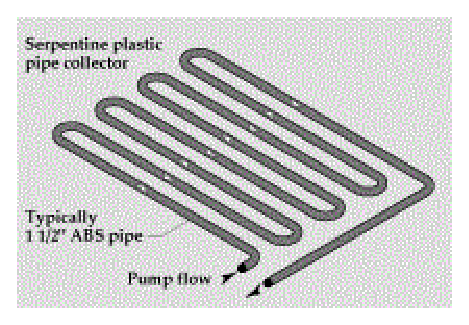
\includegraphics[keepaspectratio=true,scale=0.8]{figuras/serpentina.eps}
	\caption{Serpentina tipo painel. Fonte: Wikipedia - Site de Internet}
	\label{serpentina}
\end{figure}

Dos modelos de serpentina que serão estudados para ver qual se adequa melhor ao projeto, se tem 3 opções:

\begin{itemize}
  \item \textbf{Serpentina completamente dentro do reator:} Se escolhida essa opção o materialda serpentina será de aço inox, para evitar contaminação do mostro;
  \item \textbf{Serpentina parcialmente dentro do reator:} A serpentina passaria por pontos específicos do reator, para diminuir consideravelmente o acúmulo de mostro nos enrolamentos da estrutura;
  \item \textbf{Serpentina completamente fora do reator, em volta da parte externa:} Nesse caso teria a necessidade de adicionar um material isolante em volta da serpentina para que não houvesse interferência do ambiente na troca de calor;
\end{itemize}

Além dos sistemas citados, outra opção interessante é o uso de pastilhas termoelétricas do tipo \textit{Peltier}. Elas são um cooler termoelétrico com a capacidade de aquecer e resfriar objetos em minutos com a simples alimentação dos seus terminais. Ou seja, seu princípio de funcionamento se consiste basicamente na passagem de corrente elétrica contínua entre dois metais diferentes e com isso, aplica-se uma voltagem entre os pólos, que por consequência, um diferencial de temperatura entre as faces opostas das placas, é criado. Importante ressaltar que apesar da pastilha ter a capacidade de aquecimento, nesse projeto ela será usada apenas para resfriar, uma vez que o sistema de aquecimento é separado e controlado de forma PID.

Após ligar a pastilha \textit{Peltier} um lado irá aquecer rapidamente, enquanto o outro esfriará, contudo para que não entre em equilíbrio e comprometa a pastilha é necessário um dissipador de calor do lado quente. Essa partilha será ligada em uma fonte de 12V. A Figura \ref{pastilhas} mostra o funcionamento simplificado de como essas pastilhas funcionam, com relação a transferência de calor.

\begin{figure}[h]
	\centering
	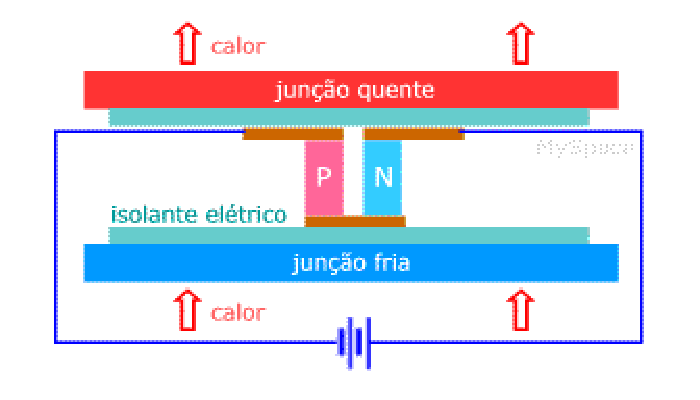
\includegraphics[keepaspectratio=true,scale=0.6]{figuras/pastilhas.eps}
	\caption{Funcionamento das pastilhas termoelétricas}
	\label{pastilhas}
\end{figure}

A figura a seguir mostra um sistema esquemático do sistema termoelétrico do efeito \textit{Peltier}, já acoplado com os respectivos dissipadores e ventiladores, componentes estes, essenciais para o adequado funcionamento do sistema.

\begin{figure}[h]
	\centering
	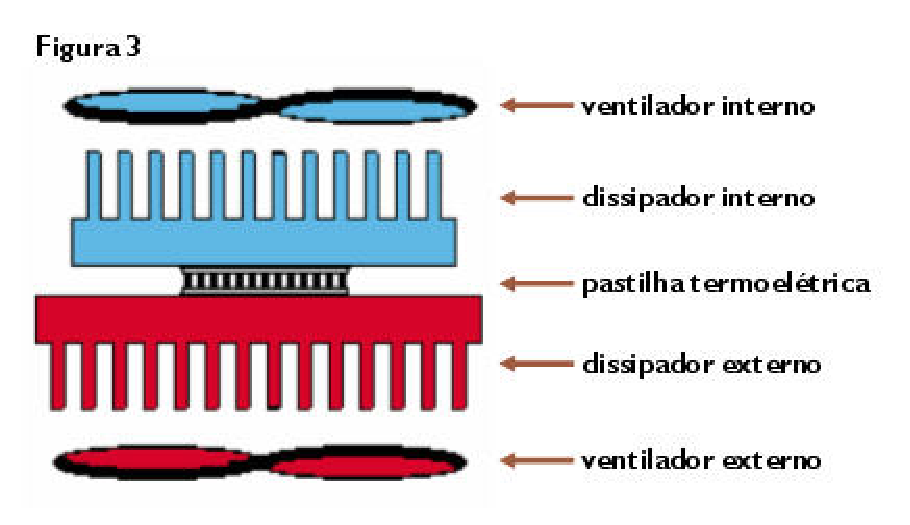
\includegraphics[keepaspectratio=true,scale=0.6]{figuras/peltier.eps}
	\caption{Esquema do efeito Peltier}
	\label{peltier}
\end{figure}

Um modelo bastante conhecido é a Pastilha Termoelétrica Peltier EC1-12706 Cooler.

\begin{figure}[h]
	\centering
	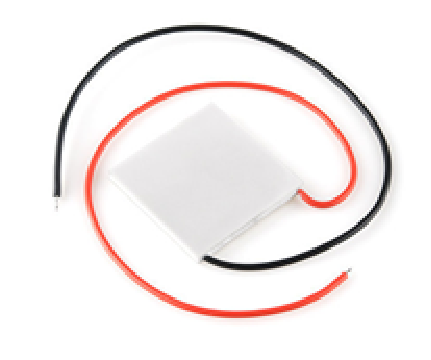
\includegraphics[keepaspectratio=true,scale=0.6]{figuras/cooler.eps}
	\caption{Pastilha Termoelétrica Peltier EC1-12706 Cooler}
	\label{cooler}
\end{figure}

Suas especificações são citadas abaixo:
\begin{itemize}
  \item Faixa de Temperatura: -30 a 70 Celsius;
  \item Tensão de operação: 0 -15,2 VDC;
  \item Corrente de operação: 0 - 6 A;
  \item Potência máxima: 60W;
  \item Dimensões: 40 x 40 mm
  \item Preço médio: R\$ 22,90
\end{itemize}

Em relação ao conjunto célula \textit{Peltier}, dissipador de calor e ventilador (ventoinha) encontrou-se duas possibilidades. A primeira seria comprar um radiador frigorífico (conjunto de resfriamento com os três respectivos elementos já montados), figura \ref{radiador}.

\begin{figure}[h]
	\centering
	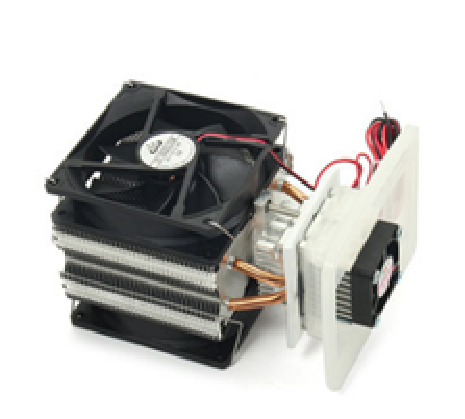
\includegraphics[keepaspectratio=true,scale=0.5]{figuras/radiador.eps}
	\caption{Radiador para refrigeração}
	\label{radiador}
\end{figure}

Em seguida ligá-lo a uma fonte de alimentação, figura \ref{radiador2}. O preço encontrado para um radiador, modelo Geekcreit® 12V 6A DIY foi em média de R\$ 68,00.

\begin{figure}[h]
	\centering
	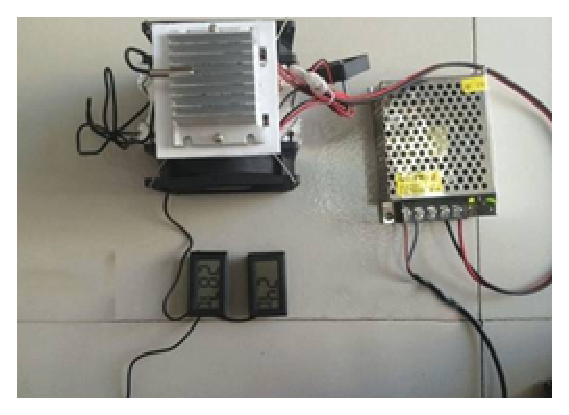
\includegraphics[keepaspectratio=true,scale=0.6]{figuras/radiador2.eps}
	\caption{Radiador conectado à fonte de 12 V}
	\label{radiador2}
\end{figure}

A segunda seria comprar os elementos separados e uni-los. Ao se realizar um estudo mais detalhado de custos a alternativa mais econômica será escolhida.

Baseando-se no uso de células \textit{Peltier} , a água em um reservatório será resfriada e esse líquido sob baixa temperatura será bombeado para que possa percorrer a serpentina que vai estar acompanhada do reator. Um modelo simplificado deste sistema é mostrado na figura \ref{resfriamento}:

\begin{figure}[h]
	\centering
	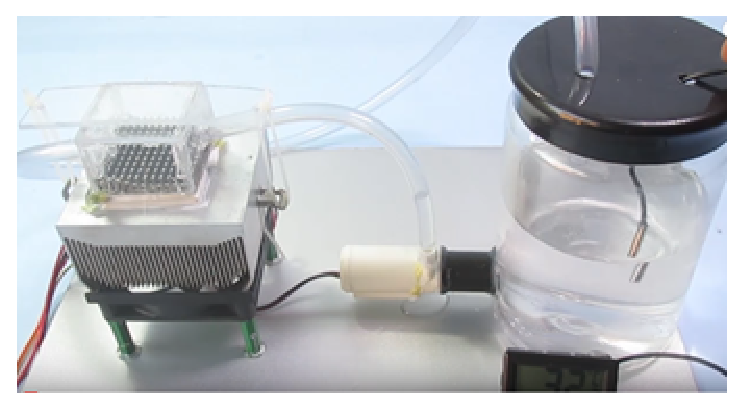
\includegraphics[keepaspectratio=true,scale=0.5]{figuras/resfriamento.eps}
	\caption{Modelo básico do sistema de resfriamento}
	\label{resfriamento}
\end{figure}

\subsubsection{Sistema de aquecimento}

Foram estudados alguns sistemas de aquecimento para o presente Biorreator e várias técnicas foram encontradas, como a  cinta térmica de silicone, que fica na parte externa à estrutura e proporciona uma transferência de calor para o fluido contido no reator, de acordo com a faixa de temperatura que se deseja, controlada através de um termostato, que oscilam de 0º a 90º ou 40º a 210º.

\begin{figure}[h]
	\centering
	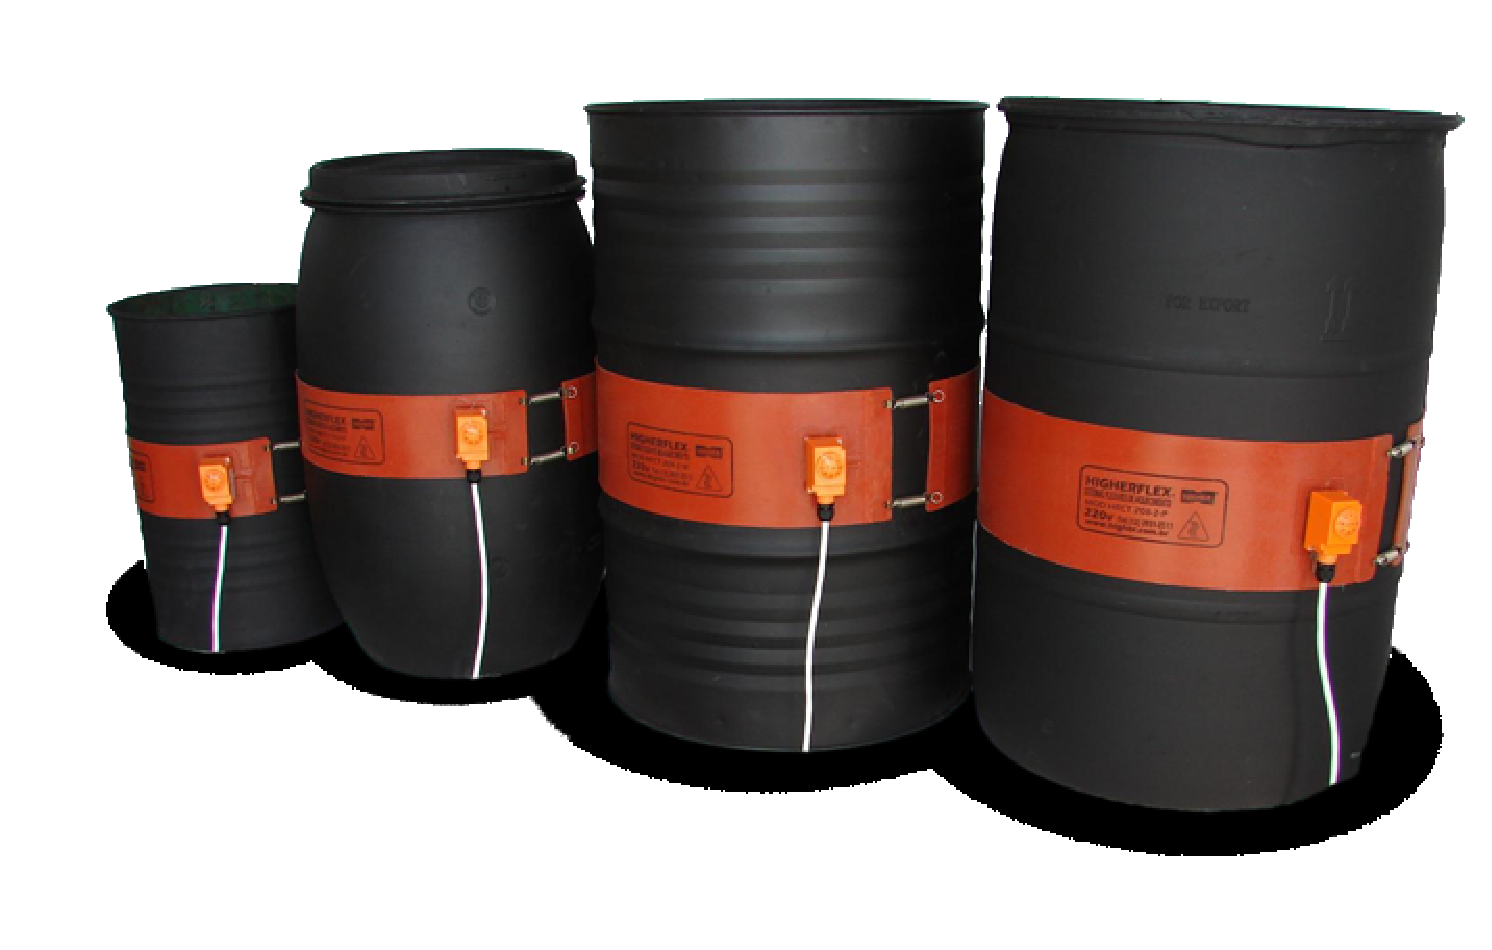
\includegraphics[keepaspectratio=true,scale=0.3]{figuras/cinta.eps}
	\caption{Modelos de cintas térmicas de silicone para diversos tamanhos de tambores}
	\label{cinta}
\end{figure}

A cinta elétrica de silicone fornece aquecimento rápido e eficaz, tendo vida útil longa e possui uma fácil aplicação, o que facilitaria o seu uso quando for necessário, já que o aquecimento seria utilizado em algumas situações específicas, pois trata-se de um biorreator genérico, onde envolverá diferentes tipos de fermentação. Este tipo de cinta é projetada para espalhar de forma eficiente o calor sobre a face do biorreator e o controle preciso de temperatura é obtido através do termostato que proporciona um aquecimento uniforme, como ilustra a Figura a seguir:

\begin{figure}[h]
	\centering
	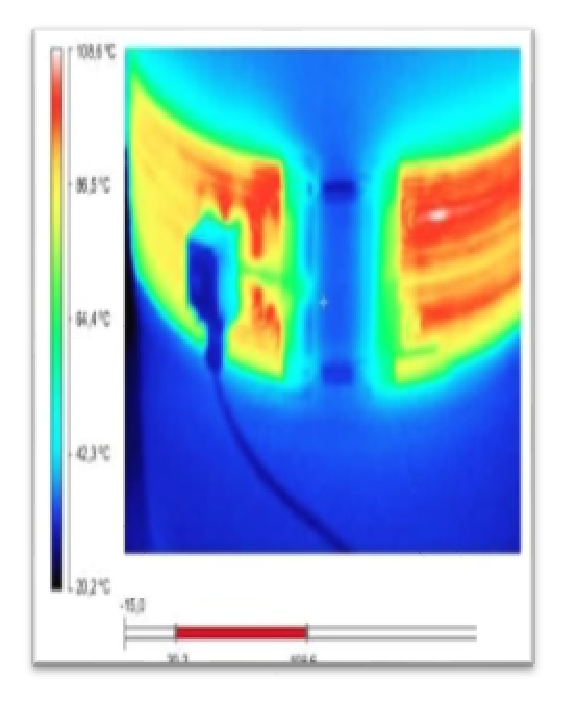
\includegraphics[keepaspectratio=true,scale=0.4]{figuras/cinta2.eps}
	\caption{Simulação de transferência de calor da cinta.
Fonte: higher.com.br}
	\label{cinta2}
\end{figure}

Outra forma que foi encontrada para o sistema de aquecimento foi a utilização de resistência elétrica para aquecer o fluido presente no reator. Essas resistências convertem energia elétrica em calor por meio do processo de dissipação de calor pelo aquecimento Joule, onde uma corrente elétrica aquece um condutor por meio da resistência inerente a ele. Um dos pontos positivos em sua utilização é que a resistência elétrica pode ser submetida a severas condições de trabalho sem prejudicar seu próprio funcionamento.

Atualmente, as resistências elétricas são constituídas de ligas de níquel e crômio que suportam temperatura de até 1000 ºC, são resistentes e também inoxidáveis.

Nas aplicações industriais, este tipo de sistema de aquecimento é mais utilizado devido a sua arquitetura de posicionamento. Em biorreatores, a resistência é utilizada pois sua instalação é feita dentro do próprio reator de forma que toda ela esteja em contato com o fluido que será aquecido, desta forma se tornou mais viável o estudo deste sistema de aquecimento, ilustrado na Figura \ref{resistencia}.

\begin{figure}[h]
	\centering
	\includegraphics[keepaspectratio=true,scale=0.2]{figuras/resistencia.eps}
	\caption{Resistência para aquecimento}
	\label{resistencia}
\end{figure}

O funcionamento do sistema de aquecimento consistirá na alimentação da resistência com corrente provinda do sistema de alimentação, para que a potência seja estabelecida e então o aquecimento aconteça. Para o controle da temperatura do fluido, o sistema de aquecimento trabalhará em conjunto com controle eletrônico na forma de controlador PID \textit{(Proporcional-Integral-Derivativo)}, que funciona como um controlador de temperatura.

 O controlador PID é integrado com um sensor de temperatura, desta forma ele calcula uma resposta de saída para a resistência, realizando assim o rampeamento da temperatura e por consequência seu controle. Os controladores PID servem para que não aconteça variação de temperatura e que a resistência mantenha o fluido em um temperatura constante. A Figura \ref{pid} ilustra um dos tipos de controladores PID.

 \begin{figure}[h]
 	\centering
 	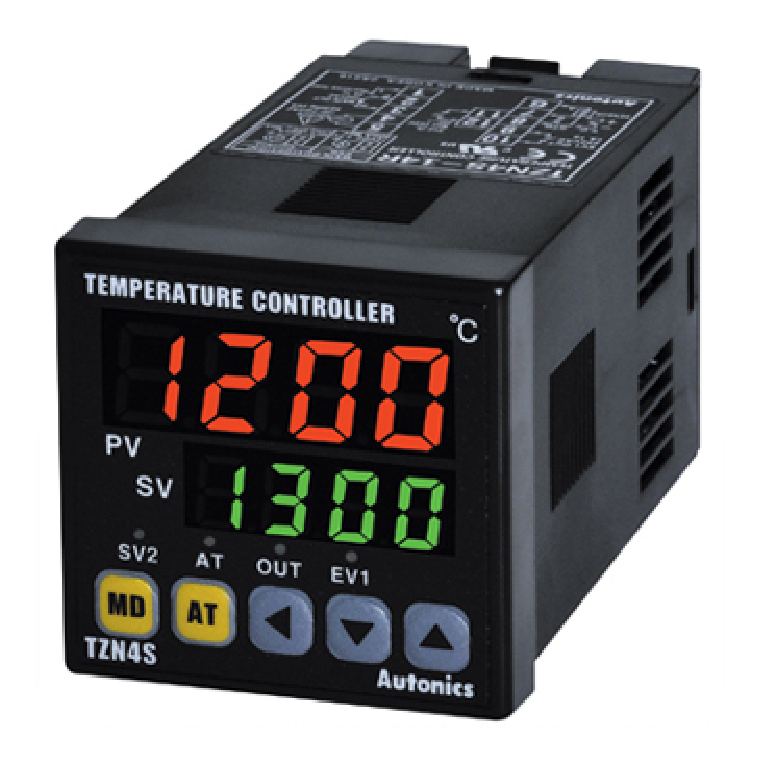
\includegraphics[keepaspectratio=true,scale=0.3]{figuras/pid.eps}
 	\caption{PID para controle de temperatura. Fonte: Ballast Conectors}
 	\label{pid}
 \end{figure}

\subsubsection{Sistema de Armazenamento de CO2}

A partir do cenário mundial, quanto a questões ambientais, o lançamento de gases poluentes no meio ambiente tem causado inúmeros prejuízos aos seres humanos. Com isso, protocolos e acordos ambientais foram criados, no decorrer dos anos, para que essas emissões fossem feitas de forma menos intensa. Devido a isto, a captura de CO2, advindos da fermentação de biorreatores, se torna extremamente importante para o meio ambiente.

O sistema de armazenamento de CO2 deste presente projeto será feito através de um outro sistema, acoplado ao biorreator, na qual o seu princípio de se consistirá na produção de microalgas em meio aquoso, através da fotossíntese. O seu funcionamento será similar ao de um aquário, onde microalgas serão colocadas na água e uma bomba (bomba de aquário) será responsável por fazer a oxigenação da mesma. Todo esse processo deverá ser feito na presença de luz, para assim ocorrer a fotossíntese.

A forma de captura deste gás gera ainda mais valores agregados a este projeto, pois as microalgas produzirão energia em forma de biomassa, viabilizando assim a produção de biocombustíveis.

\begin{figure}[h]
 \centering
 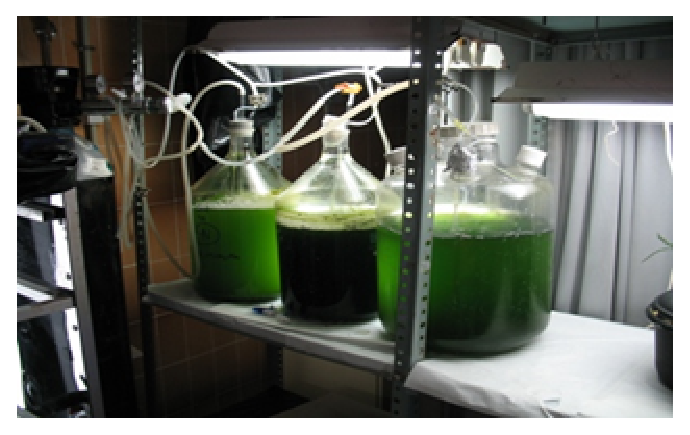
\includegraphics[keepaspectratio=true,scale=0.5]{figuras/algas.eps}
 \caption{Produção de microalgas. Fonte: dicasverdes.com}
 \label{algas}
\end{figure}

O sistema que será utilizado, acoplado ao biorreator, será similar ao mostrado na Figura \ref{algas}.

\subsubsection{Alimentação da Bancada}

A alimentação da bancada se consistirá em um cabo de energia com conexão tripolar (com fio terra) seguindo a padronização da Comissão Eletrotécnica Internacional – IEC. Constituída com uma potência de 220 V, o equivalente a 1200 W, em pleno funcionamento. Acredita-se que com todos os sensores e equipamentos que serão utilizados serão compatíveis com a alimentação informada, onde todos eles estarão interligados a este cabo de energia e a um sistema de software, que permitirá ou não o seu acionamento, de acordo com a necessidade de aplicação.

\subsection{Arquitetura}

\subsubsection{Comunicação entre os módulos}

A arquitetura de comunicação do sistema foi determinada pela disposição de módulos, sendo que para cada um existe a separação de suas responsabilidades, de forma que cada um destes cumpra uma única tarefa dentro do sistema para que exista uma melhor forma de controle e manutenção. Assim tanto a identificação de problemas no decorrer do desenvolvimento e de futuras atualizações como o trabalho paralelizado são possibilitados pela natureza de que cada um destes módulos se comporta como um serviço para o sistema como um todo.

O sistema irá possuir ao todo 6 módulos e os mesmos estão separados em 3 grupos de acordo com suas principais responsabilidades: controle, comunicação e interface. Os sensores e atuadores são os módulos presentes na área de controle, por serem responsáveis por controlar e atuar sobre os índices do sistema que serão captados. Enquanto os conversores, \textit{Raspberry} e a \textit{API} serão os módulos responsáveis pelo tratamento e comunicação de dados com o aplicativo que é a camada responsável pela apresentação e recepção de valores com o usuário final.

Os módulos serão desenvolvidos com as seguintes tecnologias:
\begin{itemize}
  \item Para comunicação e tratamento de dados vindo dos sensores através de uma interface com arduino será utilizada bibliotecas em C.
  \item Para comunicação e tratamento de dados vindo dos conversores AD/DA serão utilizadas bibliotecas em Python.
  \item Para construção da API será usado um framework javascript NodeJS e será hospedado no servidor do Heroku.
  \item O aplicativo será desenvolvido através de um framework javascript de cross-platform, React Native.
\end{itemize}

\begin{figure}[h]
 \centering
 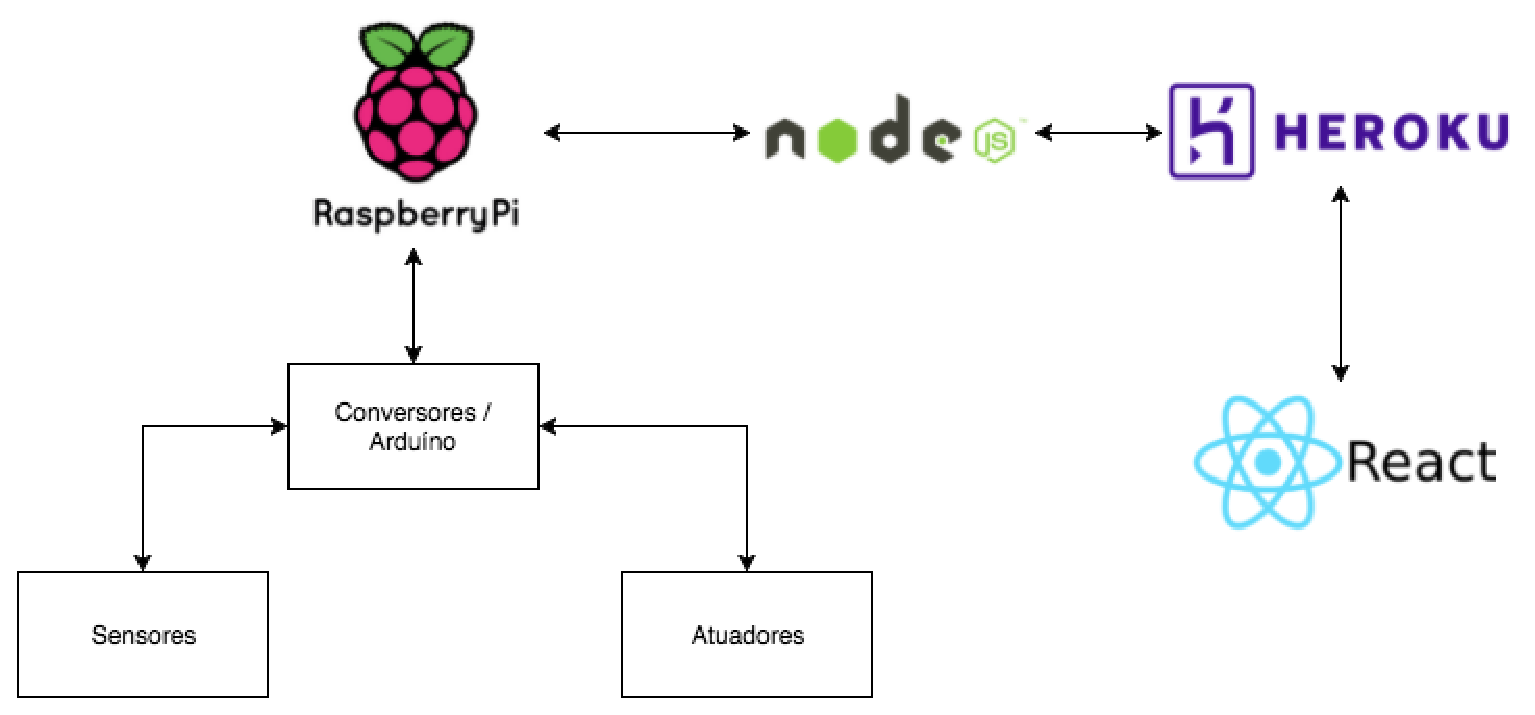
\includegraphics[keepaspectratio=true,scale=0.5]{figuras/arquitetura.eps}
 \caption{Arquitetura de monitoramento e controle}
 \label{arquitetura}
\end{figure}

\subsubsection{Especificação de Tecnologia de Software}

O sistema integrado de software terá como arquitetura duas camadas de comunicação, onde uma destas será o servidor responsável pelo tratamento e disponibilização dos dados vindos do sistema de sensores e a outra será a aplicação de interface com o usuário, onde serão apresentados gráficos e também recebidos inputs necessários para o sistema.

Para o servidor será utilizado um mecanismo de execução em Javascript, o NodeJS, que será responsável pelo serviço de \textit{REST}, que é uma abstração da arquitetura da \textit{World Wide Web} através de protocolos de comunicação \textit{HTTP} sendo aplicado à um web service fornecendo uma API para acesso do sistema de interface com o usuário. Como notação para transferência de dados será utilizado objetos \textit{JSON} para enviar as estruturas para o sistema de interface.

O sistema de interface com usuários será focado para uso mobile então será utilizado o \textit{framework} \textit{ReactNavite}, este é um \textit{cross-platform} em \textit{Javascript} que será responsável por gerar aplicativos para plataformas \textit{Android e iOS}. O aplicativo terá como função comunicar com a \textit{API} para recepção de dados que serão mostrados em relatórios ou para enviar dados que serão responsáveis por emitir sinais junto aos atuadores.
